\documentclass{beamer}

\usepackage[utf8]{inputenc}
\usepackage{csquotes}
\usepackage{latexsym,amsmath,xcolor,multicol,booktabs,calligra, animate, subfig}
\usepackage{graphicx,pstricks,listings,stackengine, bbm}
\usepackage{tikz}
\usetikzlibrary{fit,tikzmark}   
\usepackage{booktabs,cellspace}
\usepackage{color, colortbl}
\usepackage{hyperref}
\usepackage{color}
%Information to be included in the title page:
\title{Analysis of New Mexico's Financial Assurance Regulations}
\author{Lauren Beatty\\ \href{mailto:lbeatty@edf.org}{lbeatty@edf.org}}
\institute{Environmental Defense Fund}
\date{September 21, 2023}
\logo{
\includegraphics[height=1cm]{EDF_color_webRGB_2022 (2).png}\hspace*{.03\paperwidth}\vspace{.01\paperwidth}}


%Color Pallete
\definecolor{EDFblue}{RGB}{0.0, 51, 204}
\definecolor{EDFgreen}{RGB}{0, 153, 51} 
\definecolor{EDFlightgreen}{RGB}{161, 226, 20}
\definecolor{EDFcyan}{RGB}{51,204,255}
\setbeamercolor{structure}{fg=EDFblue} 
\setbeamercolor{button}{bg=EDFblue,fg=white}
\setbeamertemplate{navigation symbols}{}

\hypersetup{colorlinks,linkcolor=EDFblue,urlcolor=EDFblue}


\begin{document}

\frame{\titlepage}

\begin{frame}
\frametitle{Does the Proposed Regulation Sufficiently Cover Plugging Liabilities?}
    \begin{enumerate}
        \item Compare hypothetical bond amounts by firm against estimated well plugging costs.
        \item Analyze which blanket amounts leave the highest difference between FA amounts and plugging liabilities.
    \end{enumerate}
    Summary of findings:
    \begin{itemize}
        \item Current bonding amounts don't sufficiently cover potential plugging liabilities.
        \item In particular, individual well bonding amounts and active well blanket bonds appear too low.
    \end{itemize}
\end{frame}

\begin{frame}{Methods/Assumptions}
\label{BondCalc}
\vspace{-0.2cm}
\begin{itemize}
    \item To calculate firm-level bonds I tally the number of wells each firm has on private and state lands by well status (TA, non-TA).
    \item To calculate estimated plugging costs I assume that each well costs $\$12$ per foot to plug
\end{itemize}
\end{frame}


\begin{frame}{Current bonding don't cover potential plugging liabilities.}
\label{Fig1}
\begin{columns}
          \column{0.6\linewidth}
             \centering
             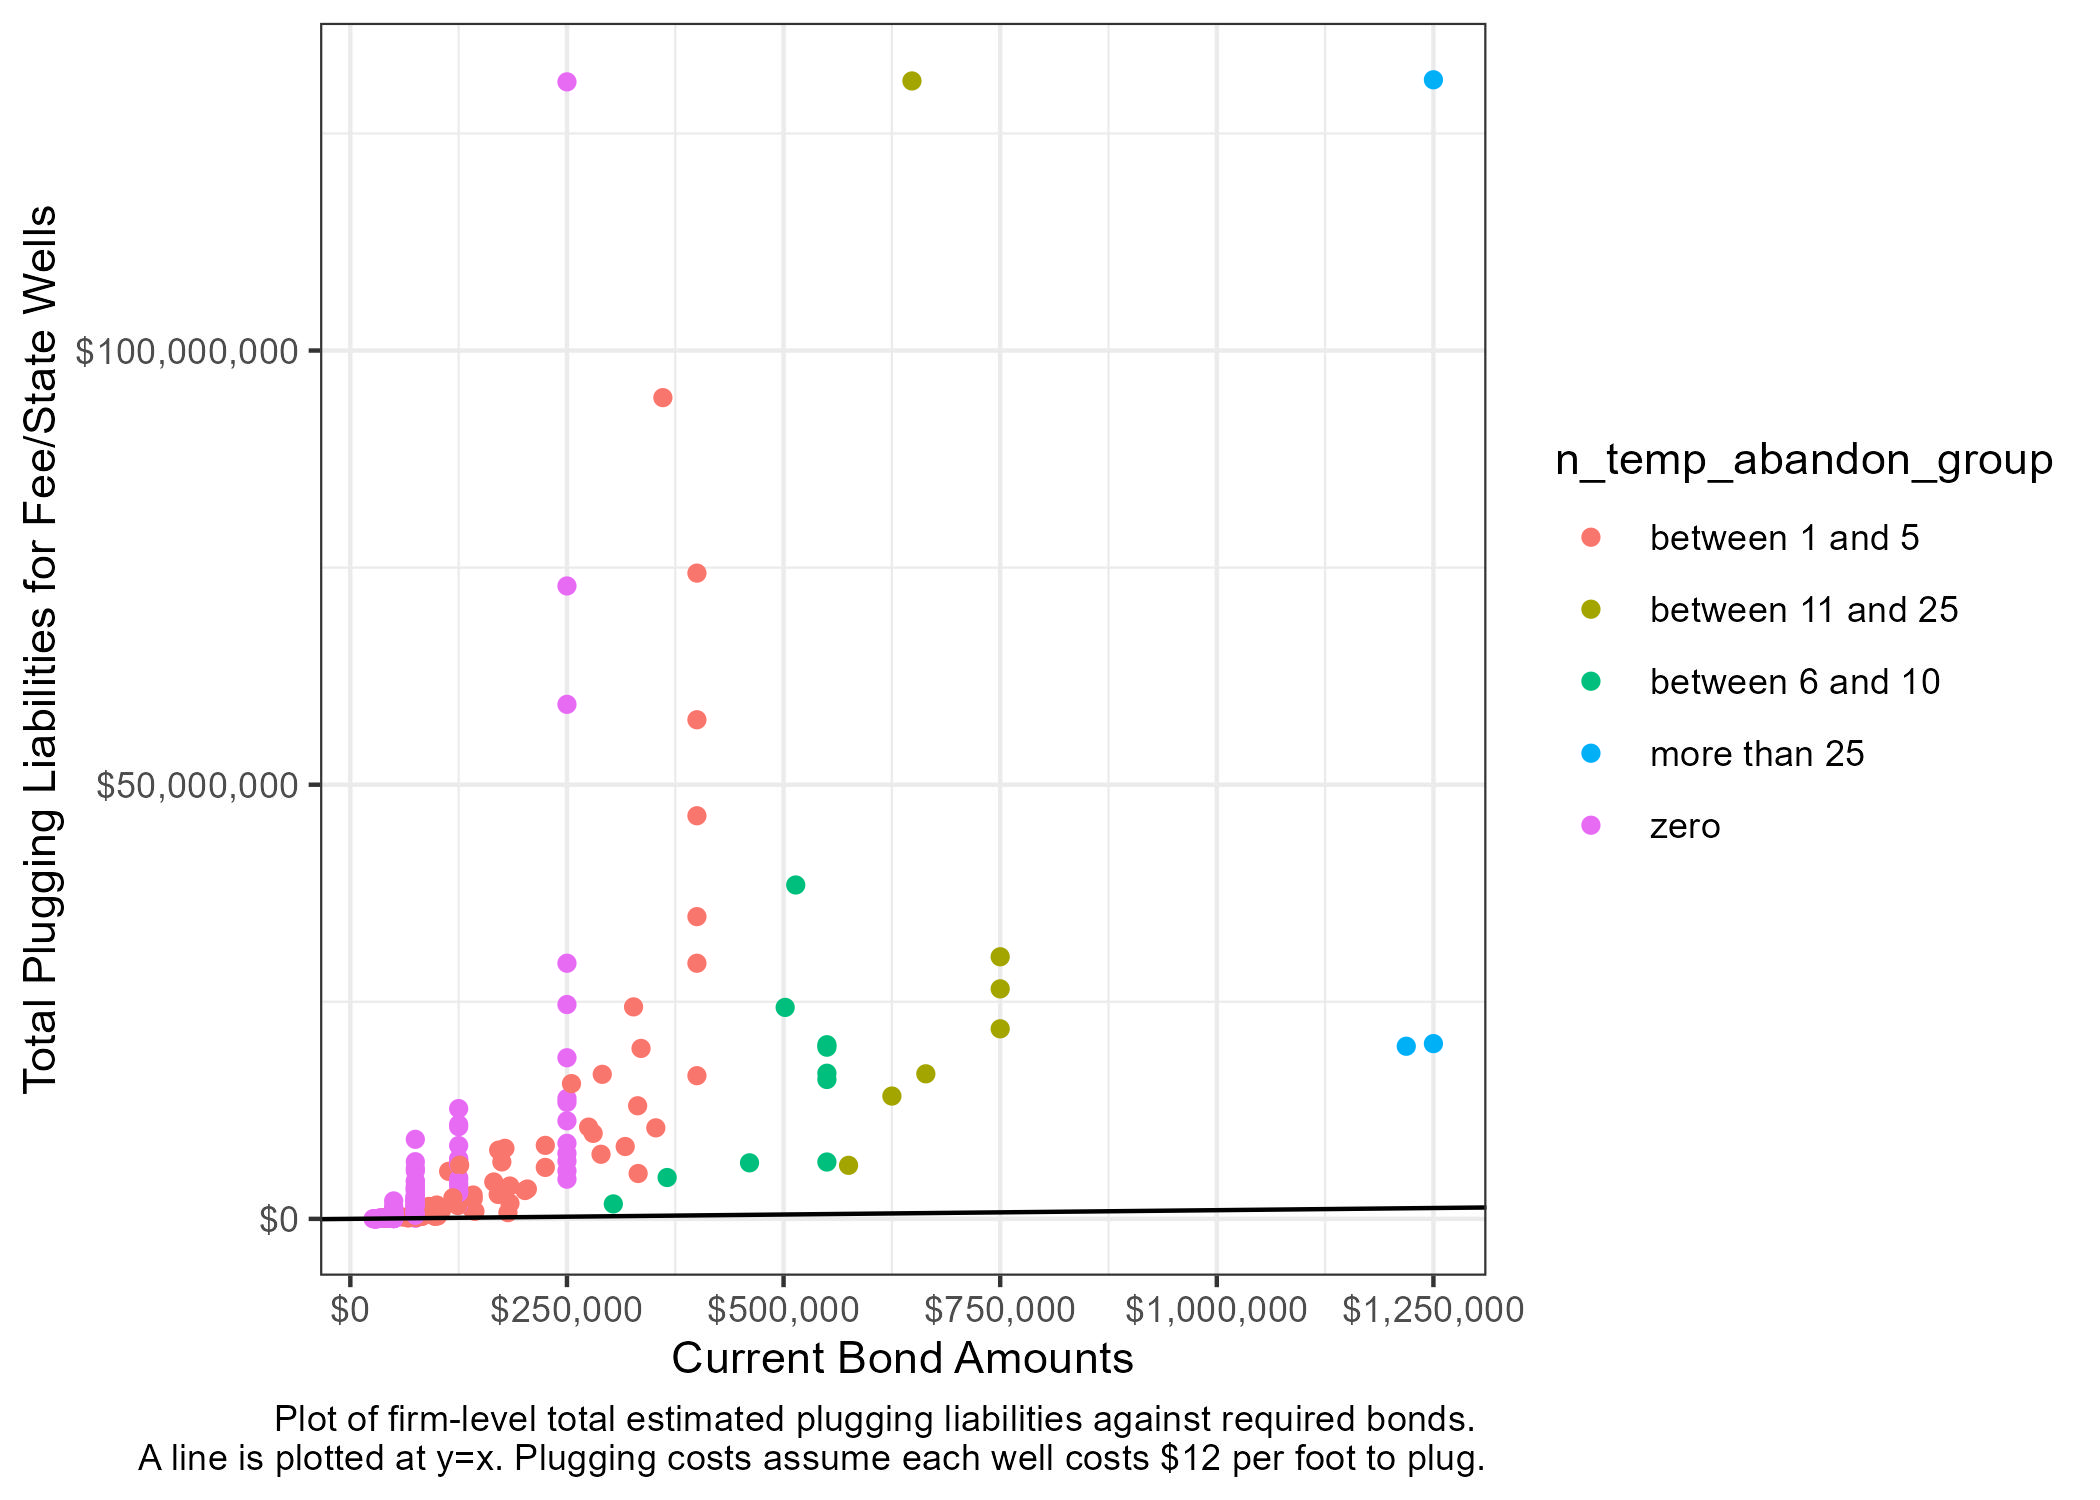
\includegraphics[width=1.08\textwidth]{Figures/CurrentBond_v_Costs.jpg}
           \column{0.5\linewidth}
              \begin{itemize}
                  \item Dots above the line represent firms whose plugging liabilities exceed bonding amounts.\
                  \item My firms have tens of millions of dollars in potential plugging liabilities and are bonded for less than one million.
              \end{itemize}
\end{columns} 
\vspace{1cm}
\end{frame}

\begin{frame}{Tripling the active bond blanket and doubling the TA blanket improves but does not fix the problem}
\vspace{-.3cm}
    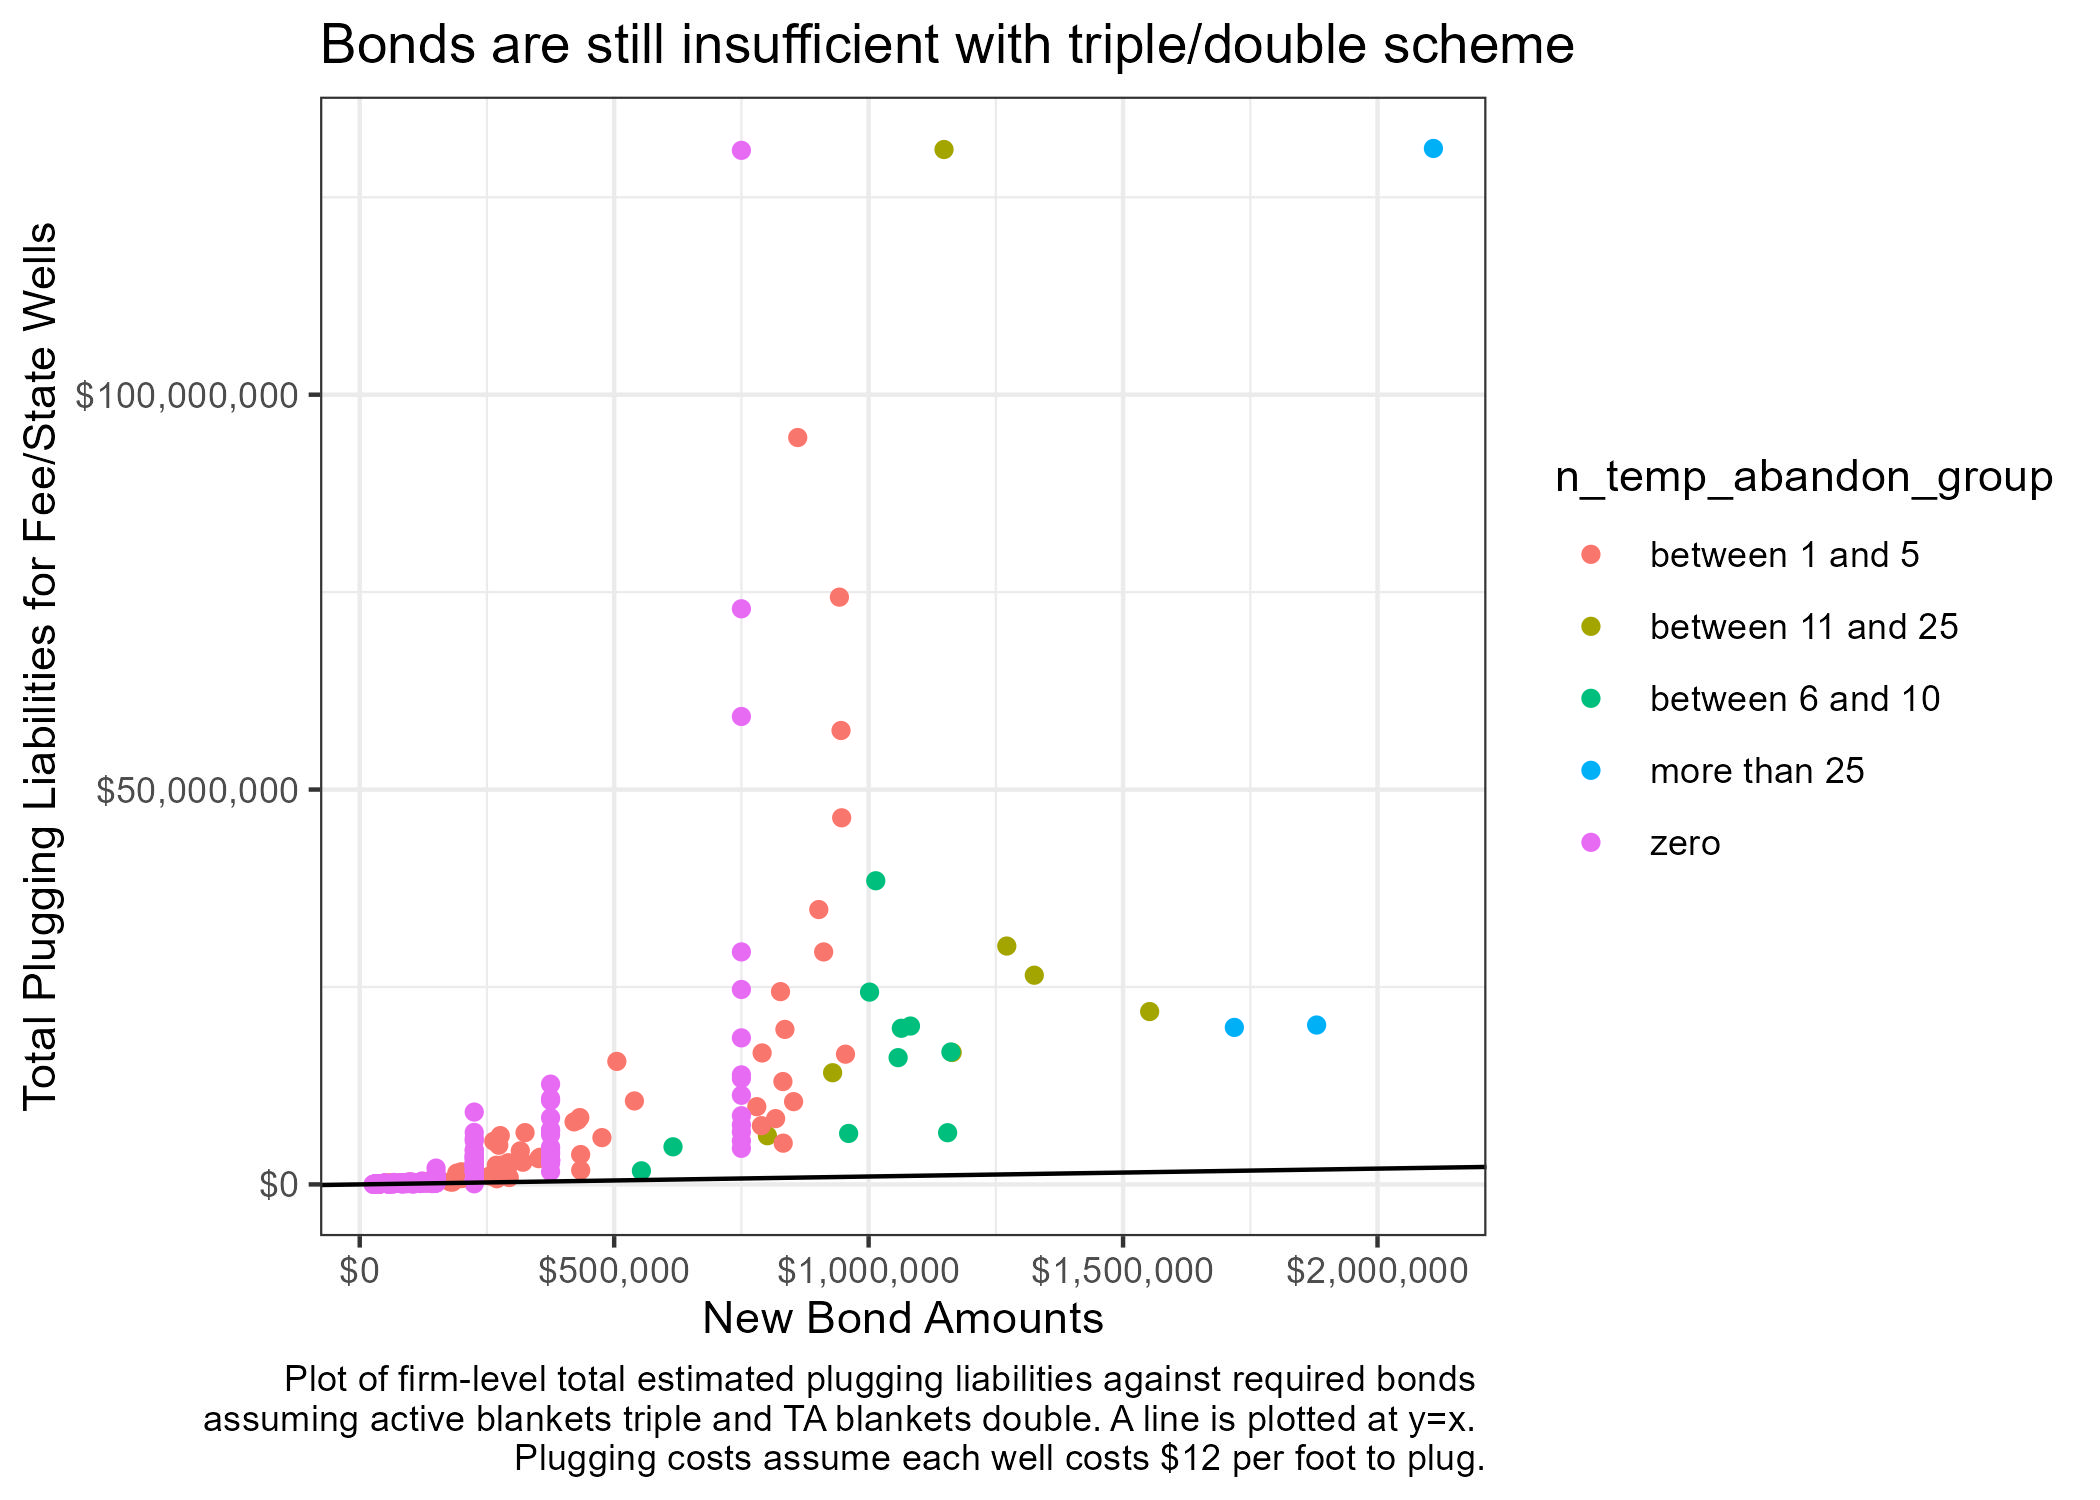
\includegraphics[width=0.8\linewidth]{Figures/TripleDoubleBond_v_Costs.jpg}
\end{frame}

\begin{frame}{Even if we just consider liabilities for marginal wells, large blankets still appear insufficient}
\vspace{-.3cm}
    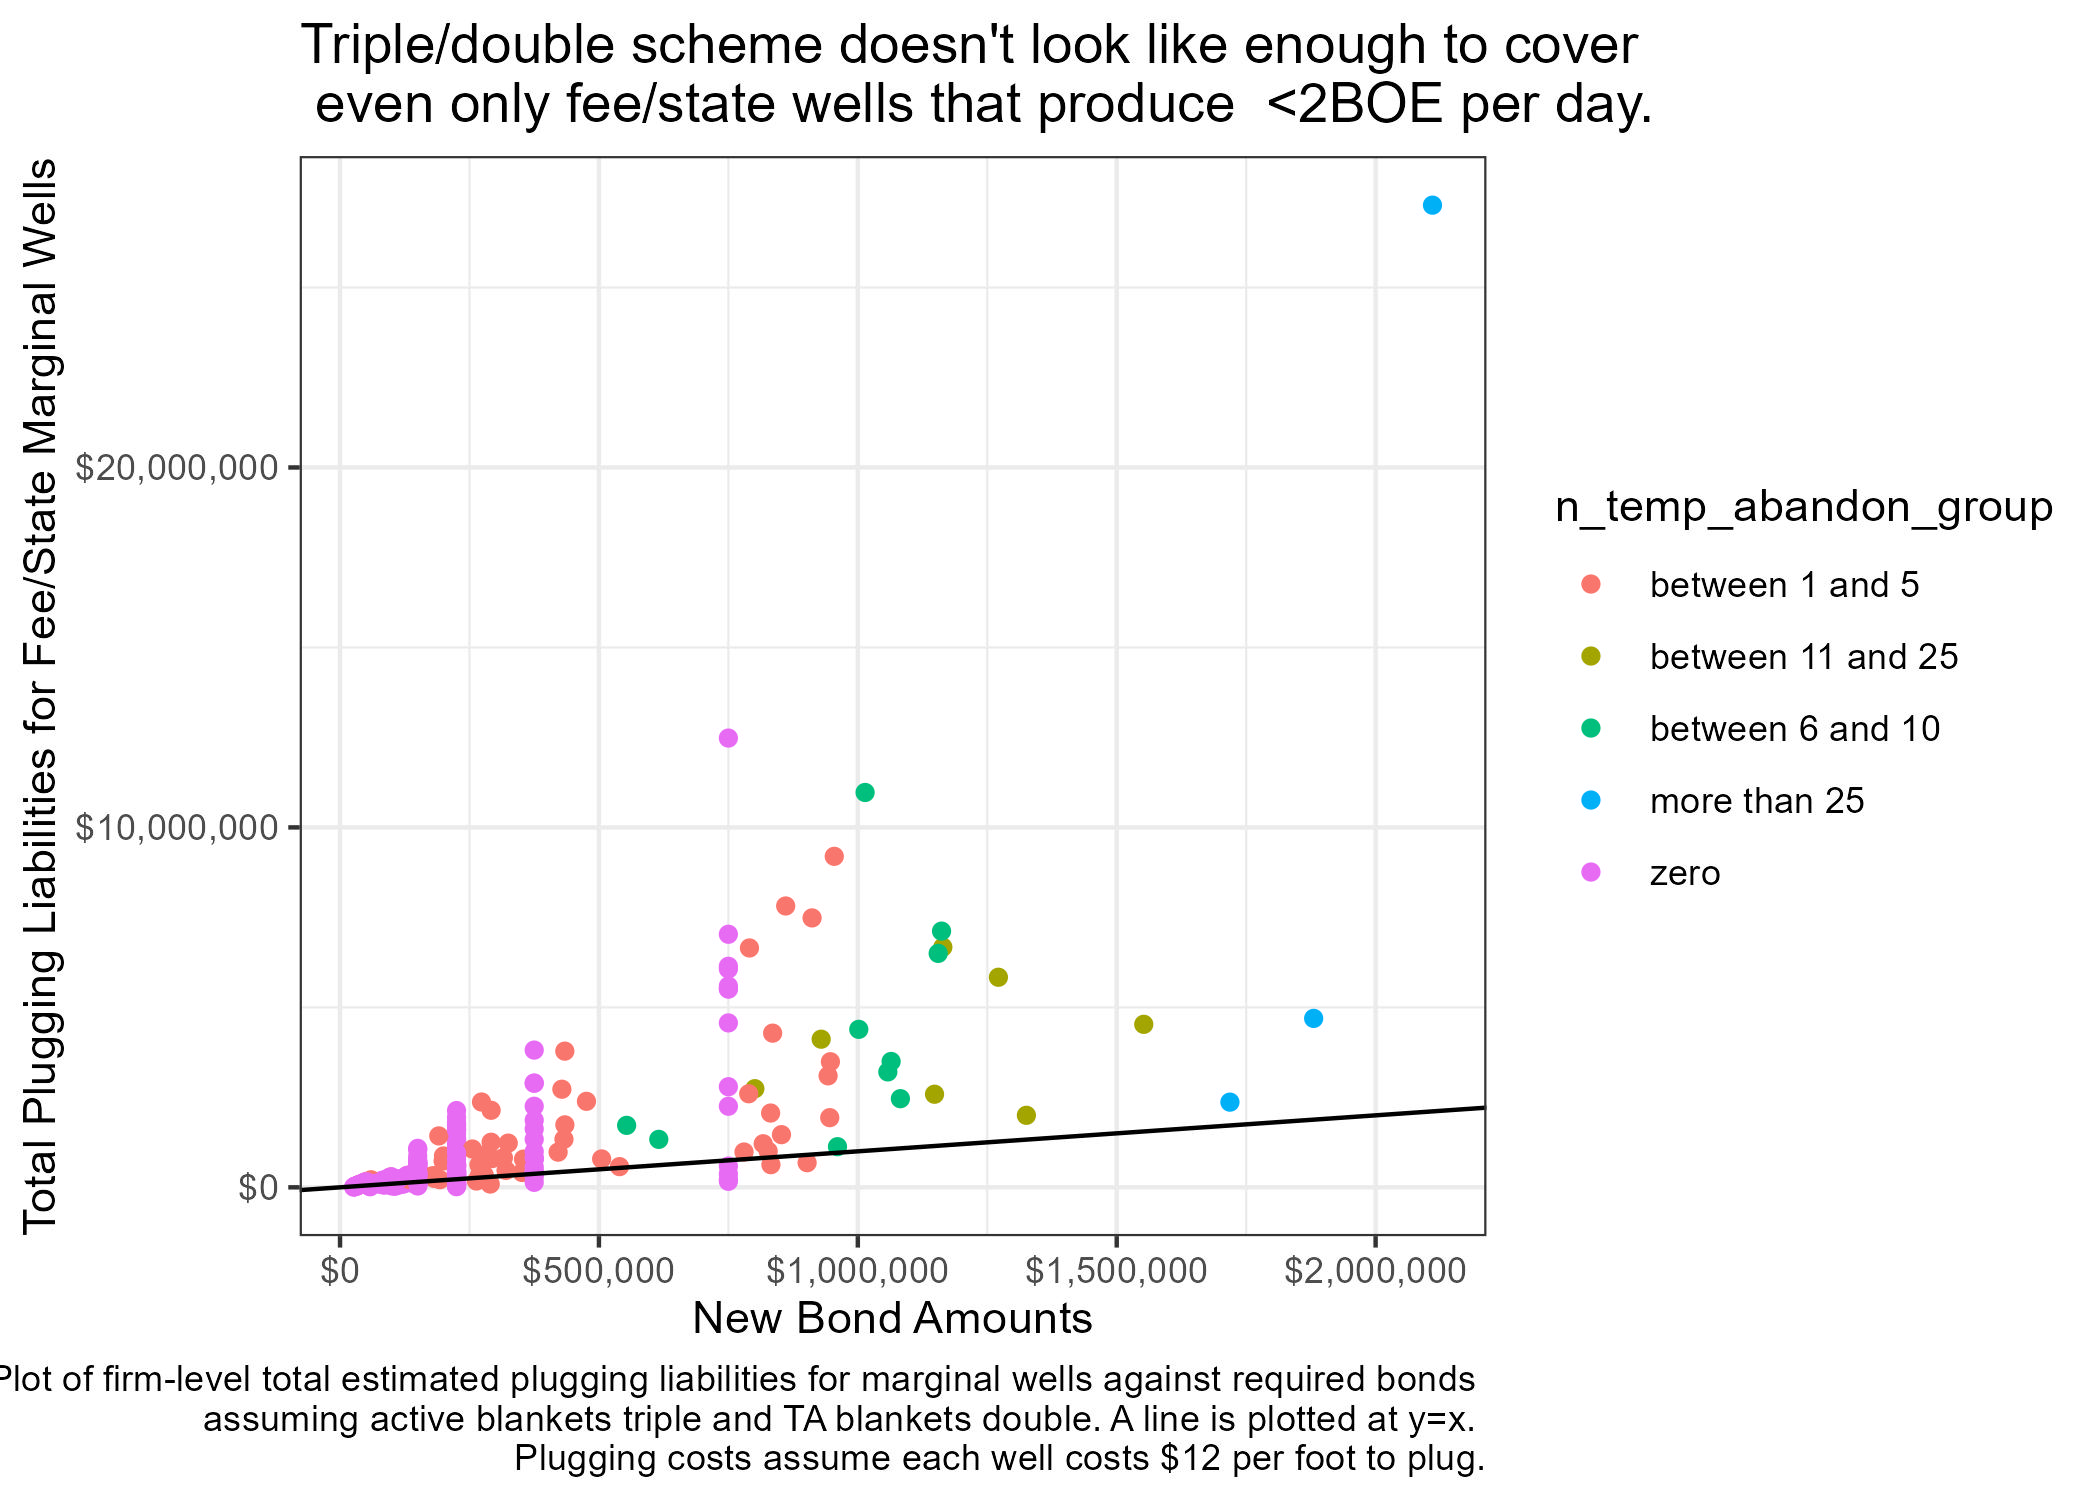
\includegraphics[width=0.8\linewidth]{Figures/TripleDoubleBond_v_MarginalCosts.jpg}
\end{frame}


\begin{frame}{Individual Well Bonds Appear Lower Than Plugging Costs}
\label{Fig2}
\vspace{-0.5cm}
\centering
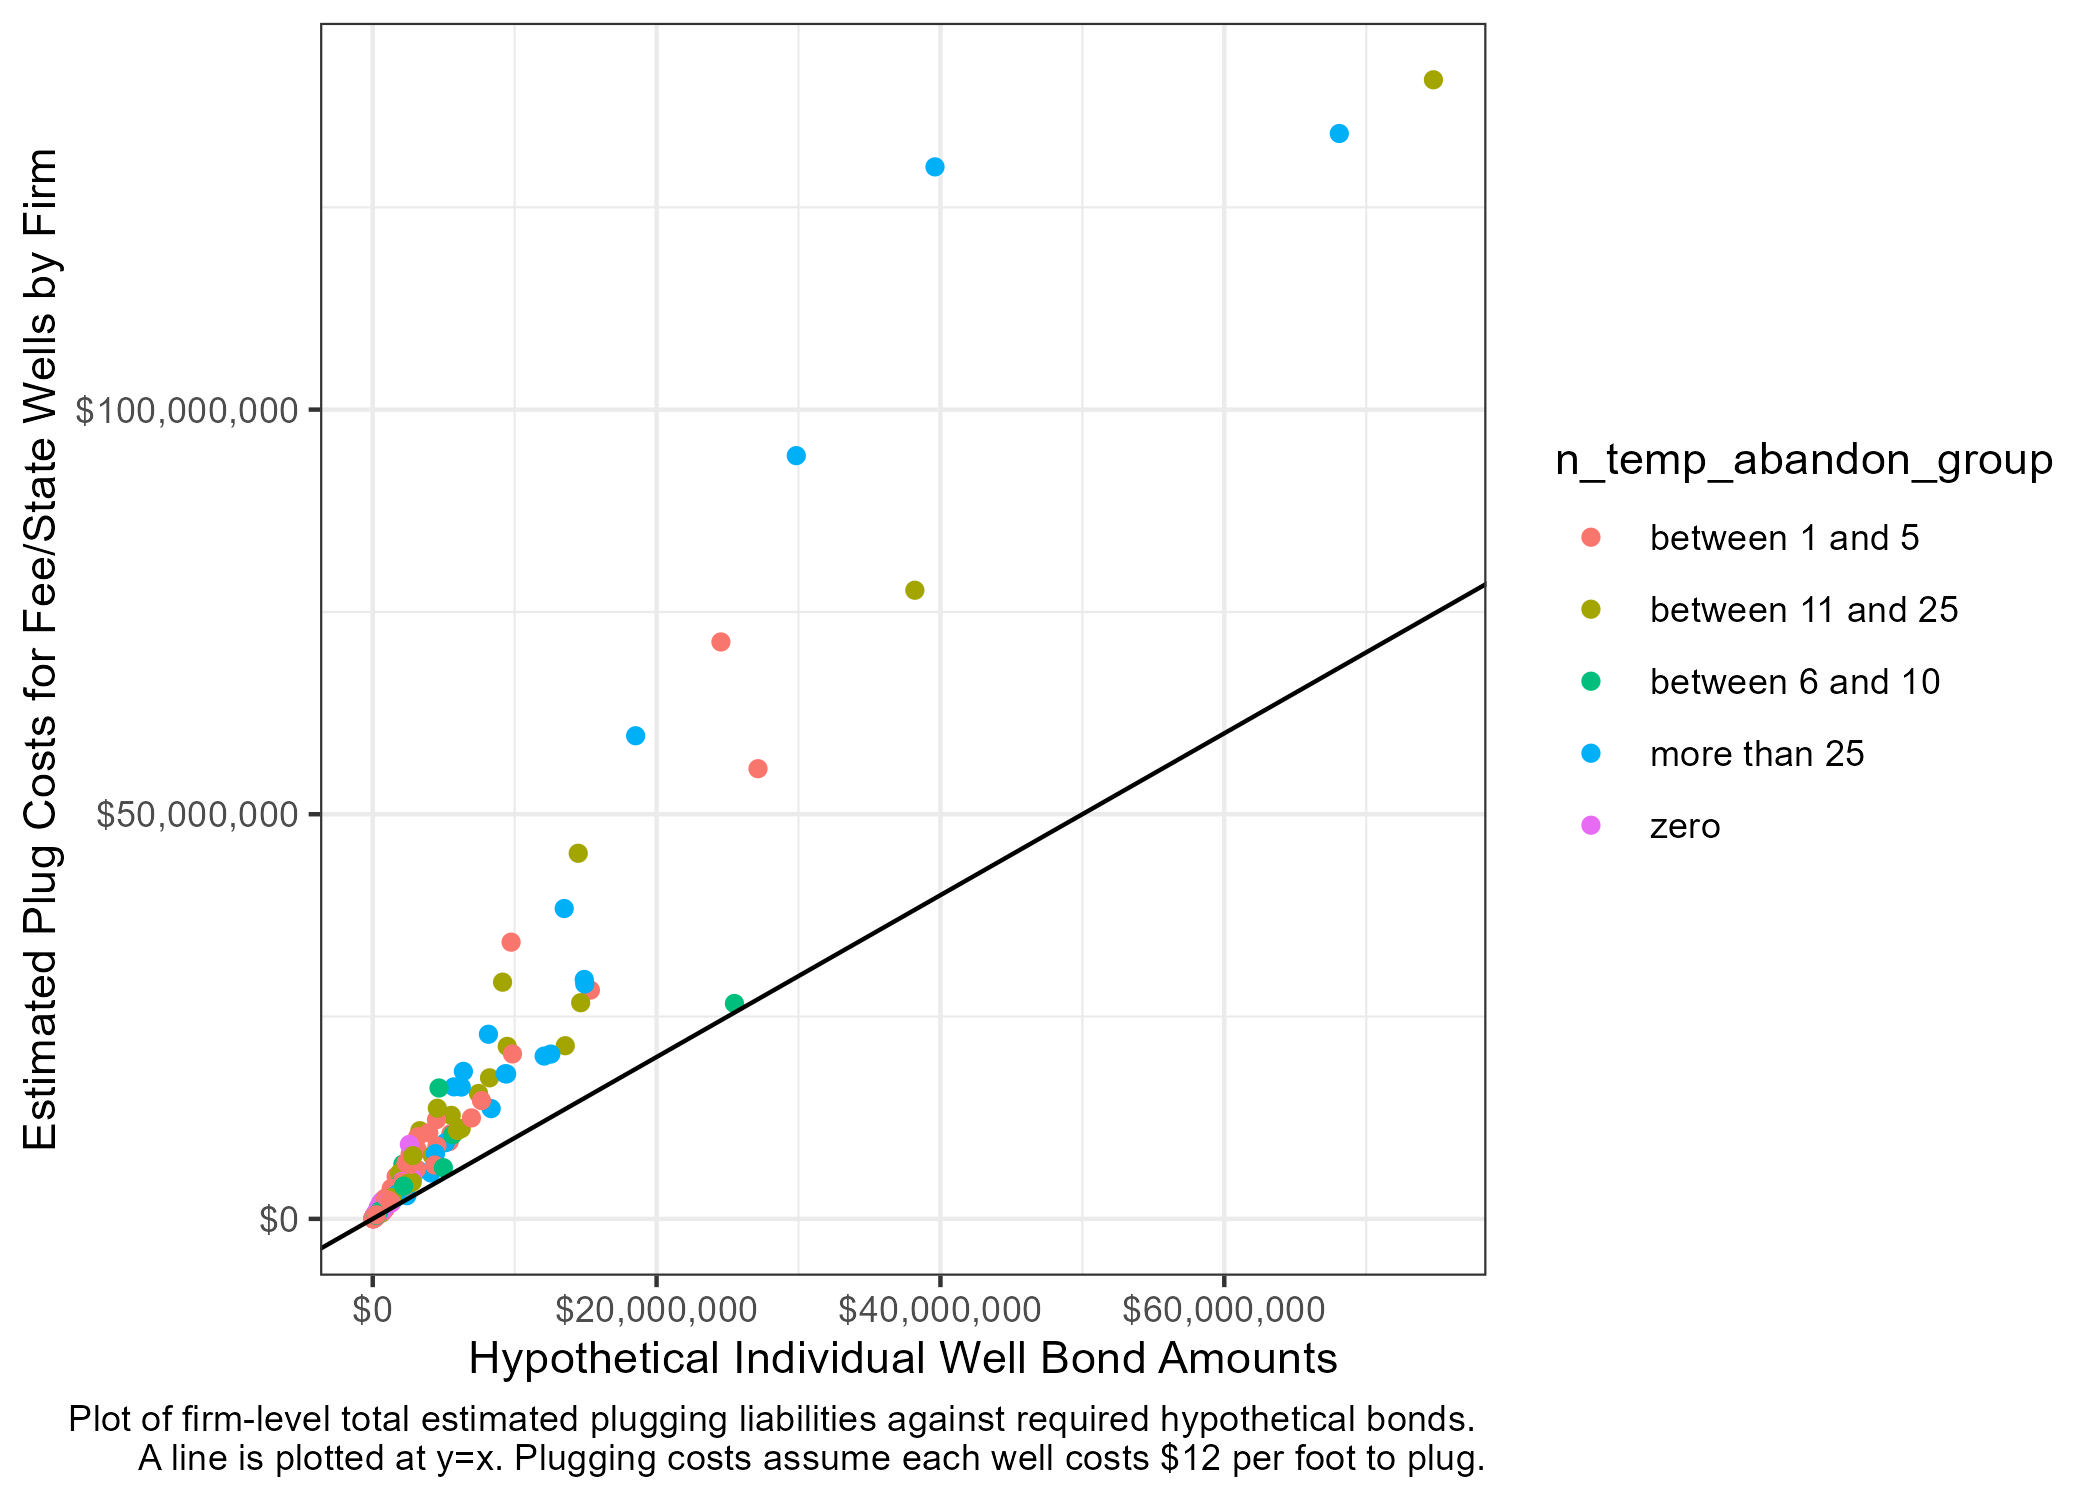
\includegraphics[width=0.8\textwidth]{Figures/PerFoot_v_Costs.jpg}    
\end{frame}

\begin{frame}{Some blankets are more problematic than others}
\vspace{-1cm}
\begin{tabular}{cc}
    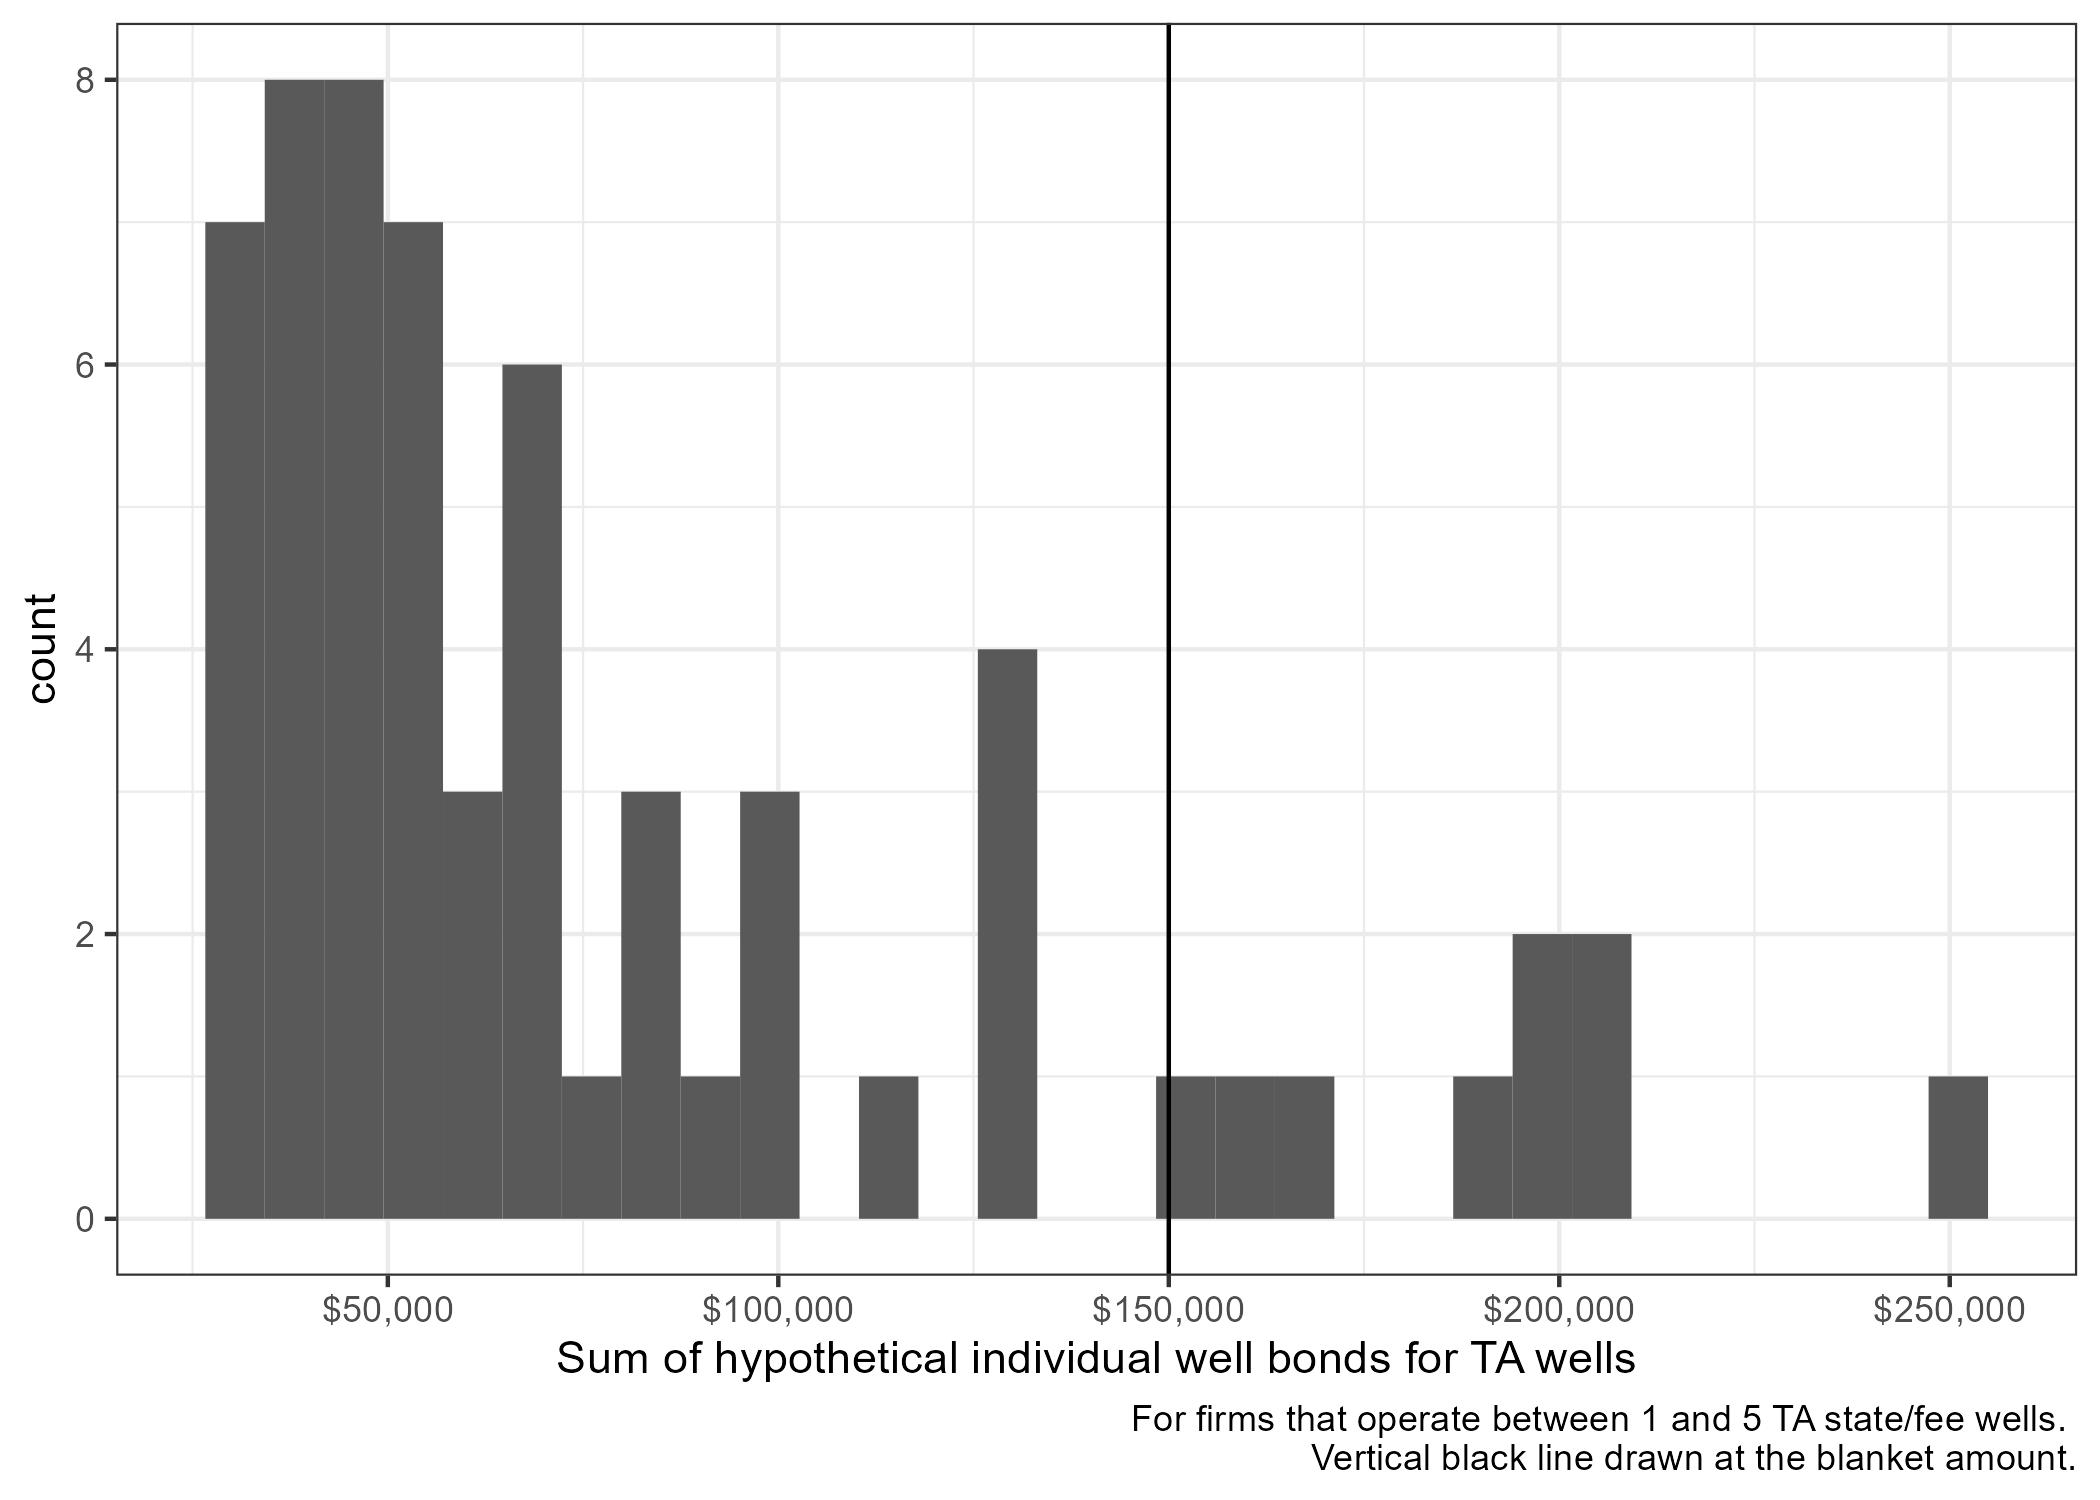
\includegraphics[width=0.45\linewidth]{Figures/Histogram_TA_1_5.jpg} & 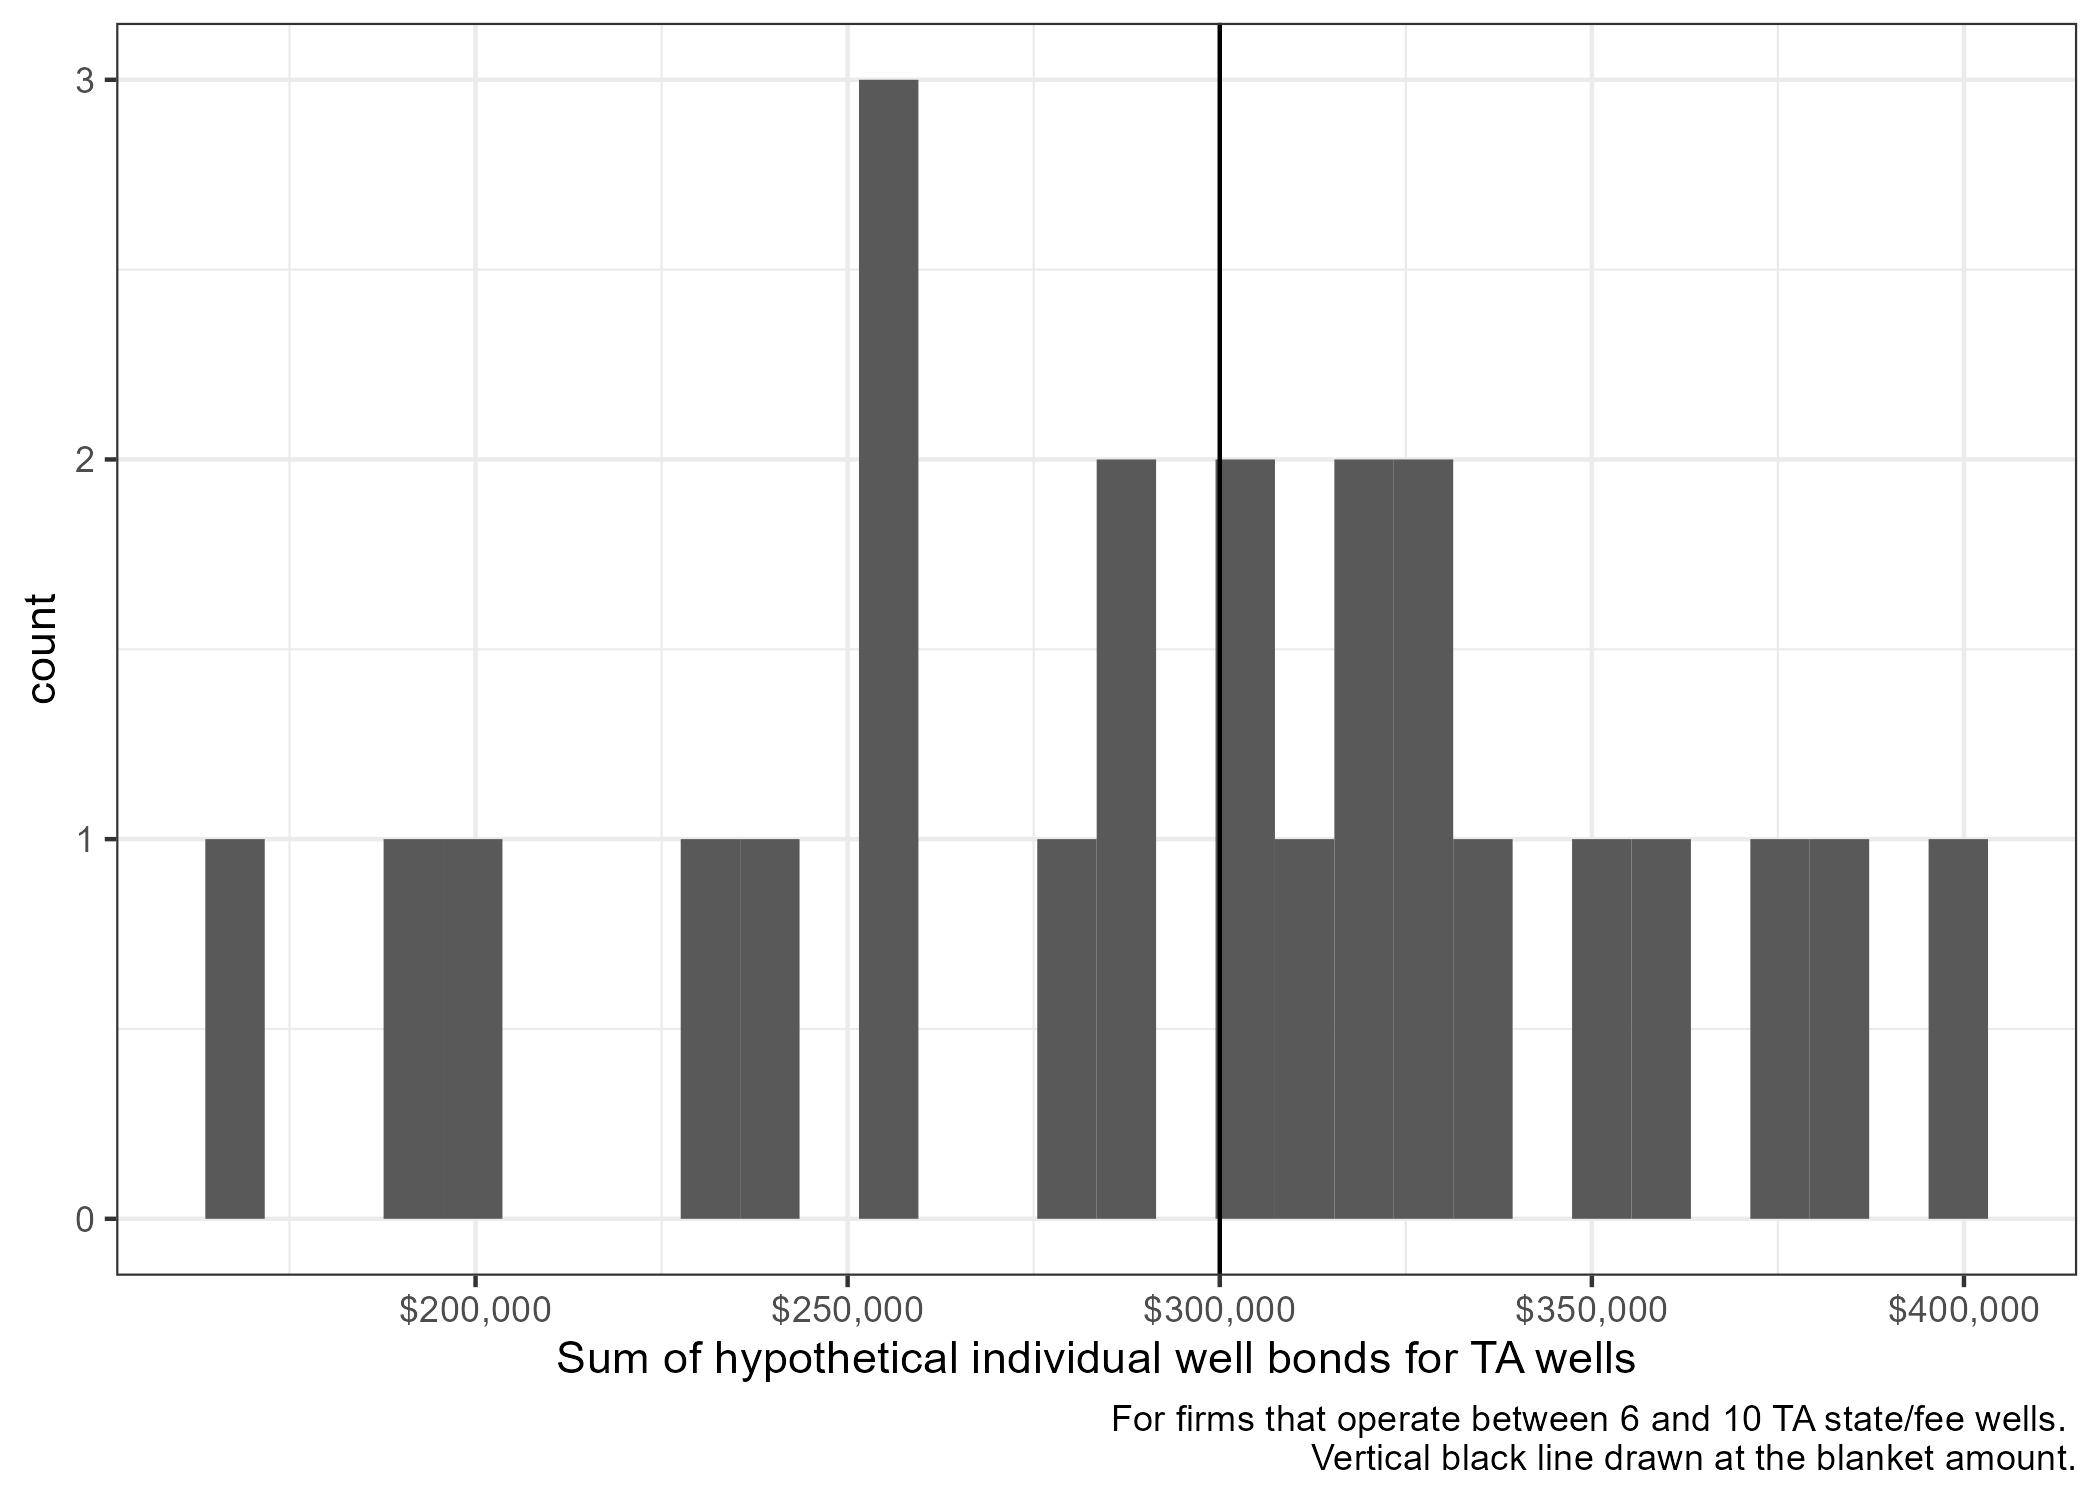
\includegraphics[width=0.45\linewidth]{Figures/Histogram_TA_6_10.jpg} \\
     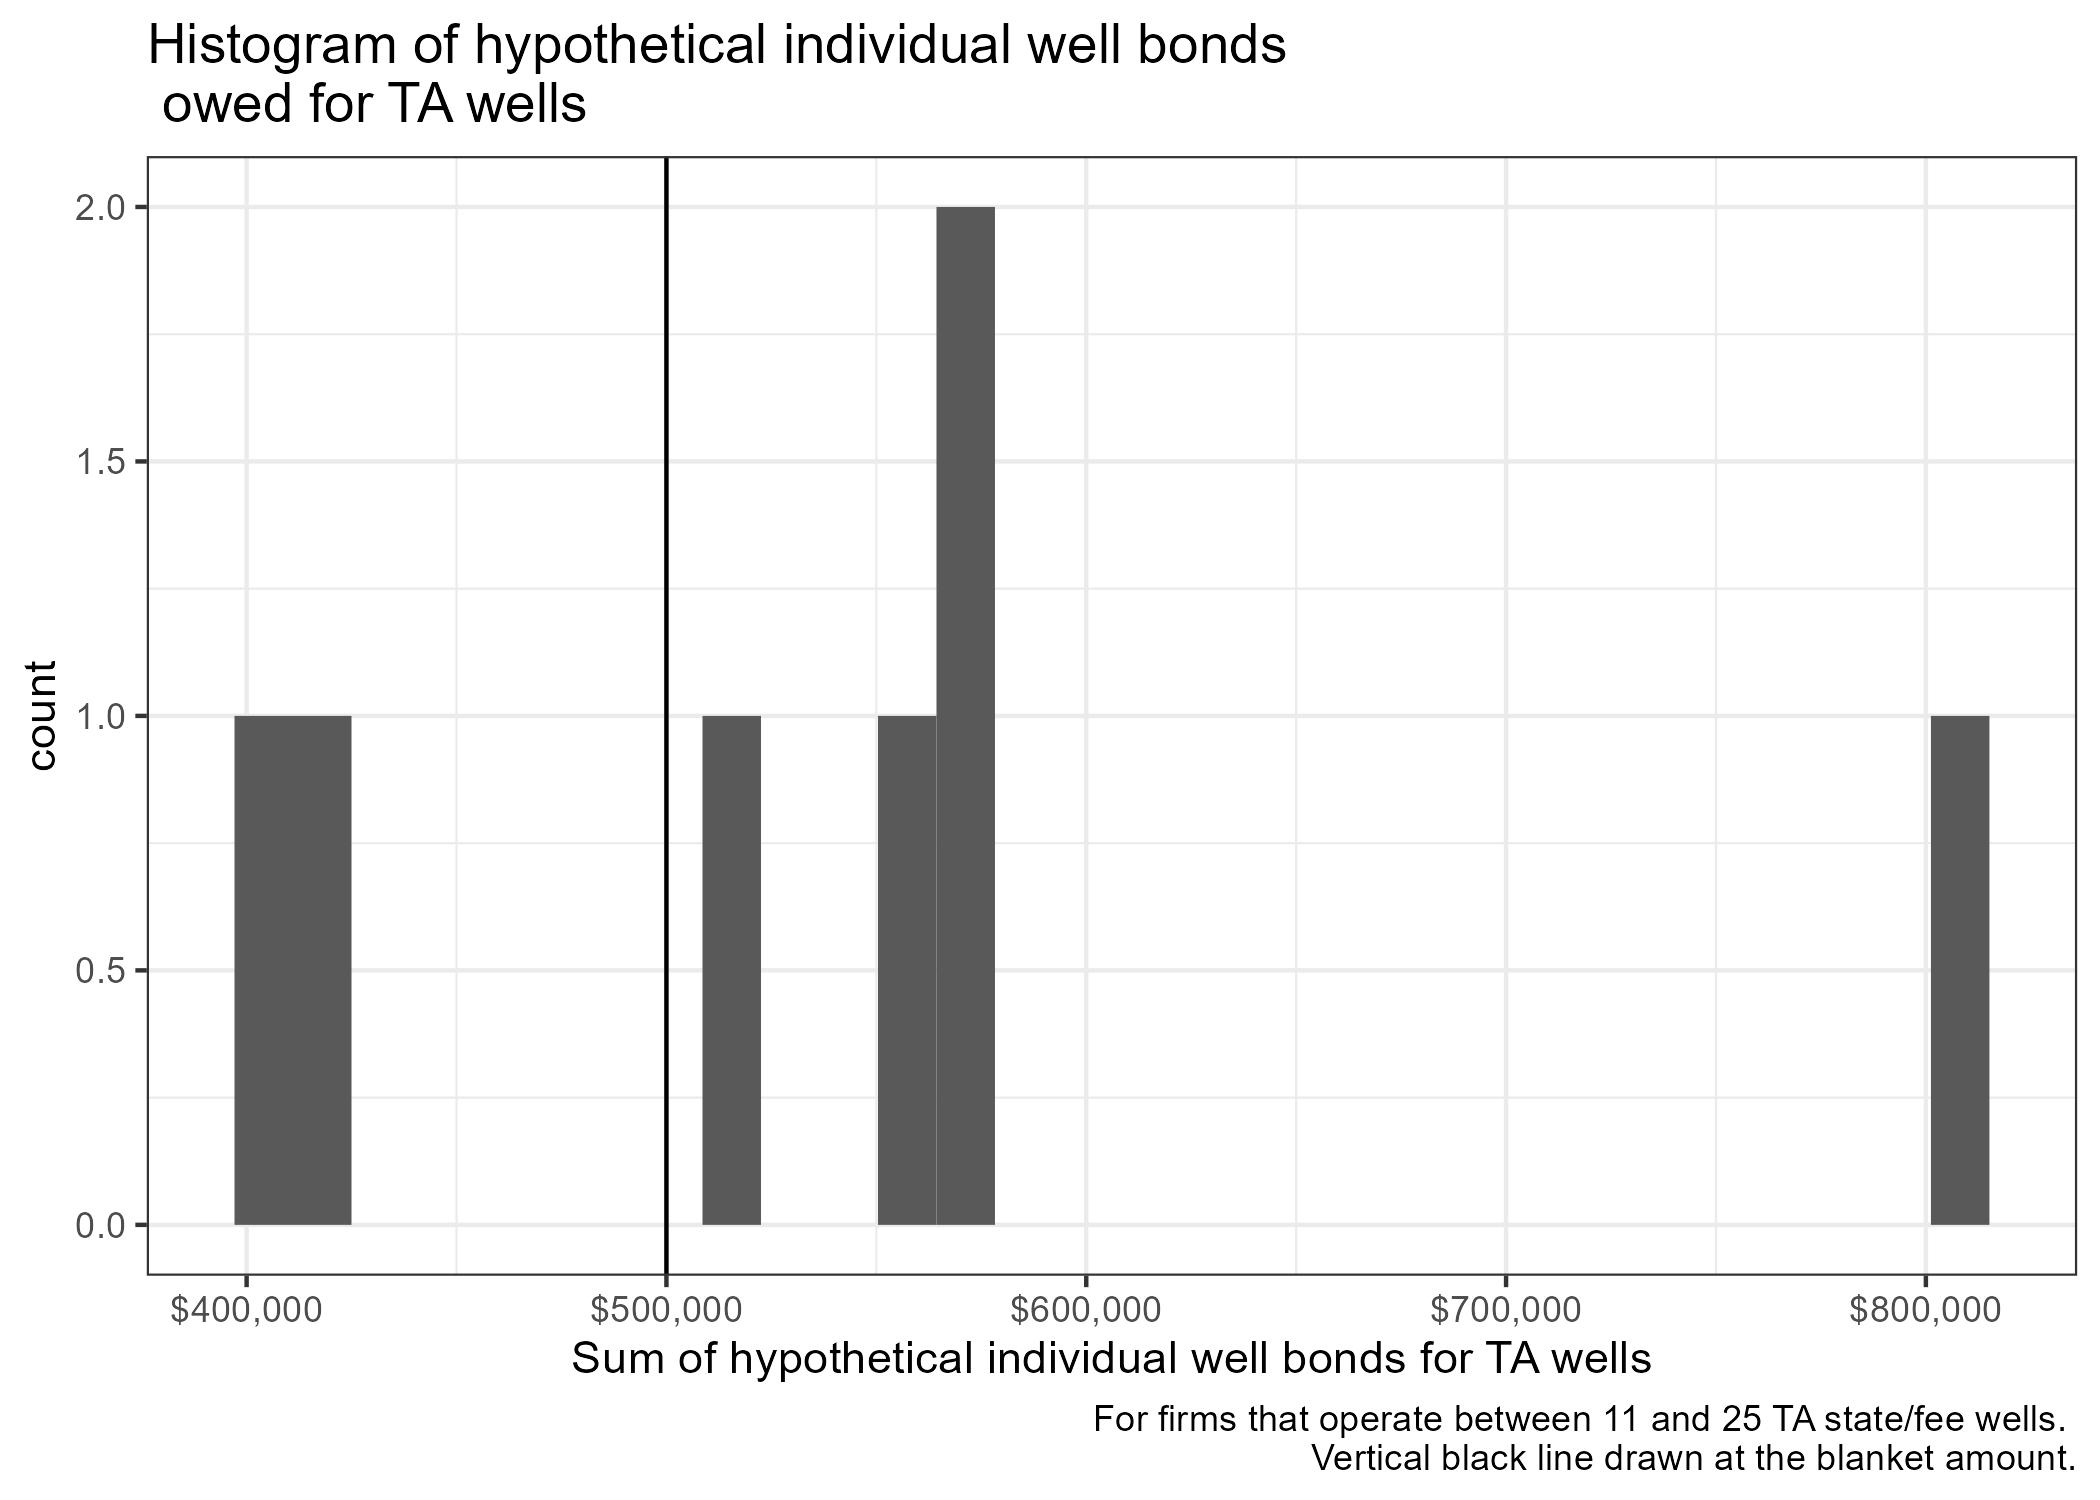
\includegraphics[width=0.45\linewidth]{Figures/Histogram_TA_11_25.jpg}& 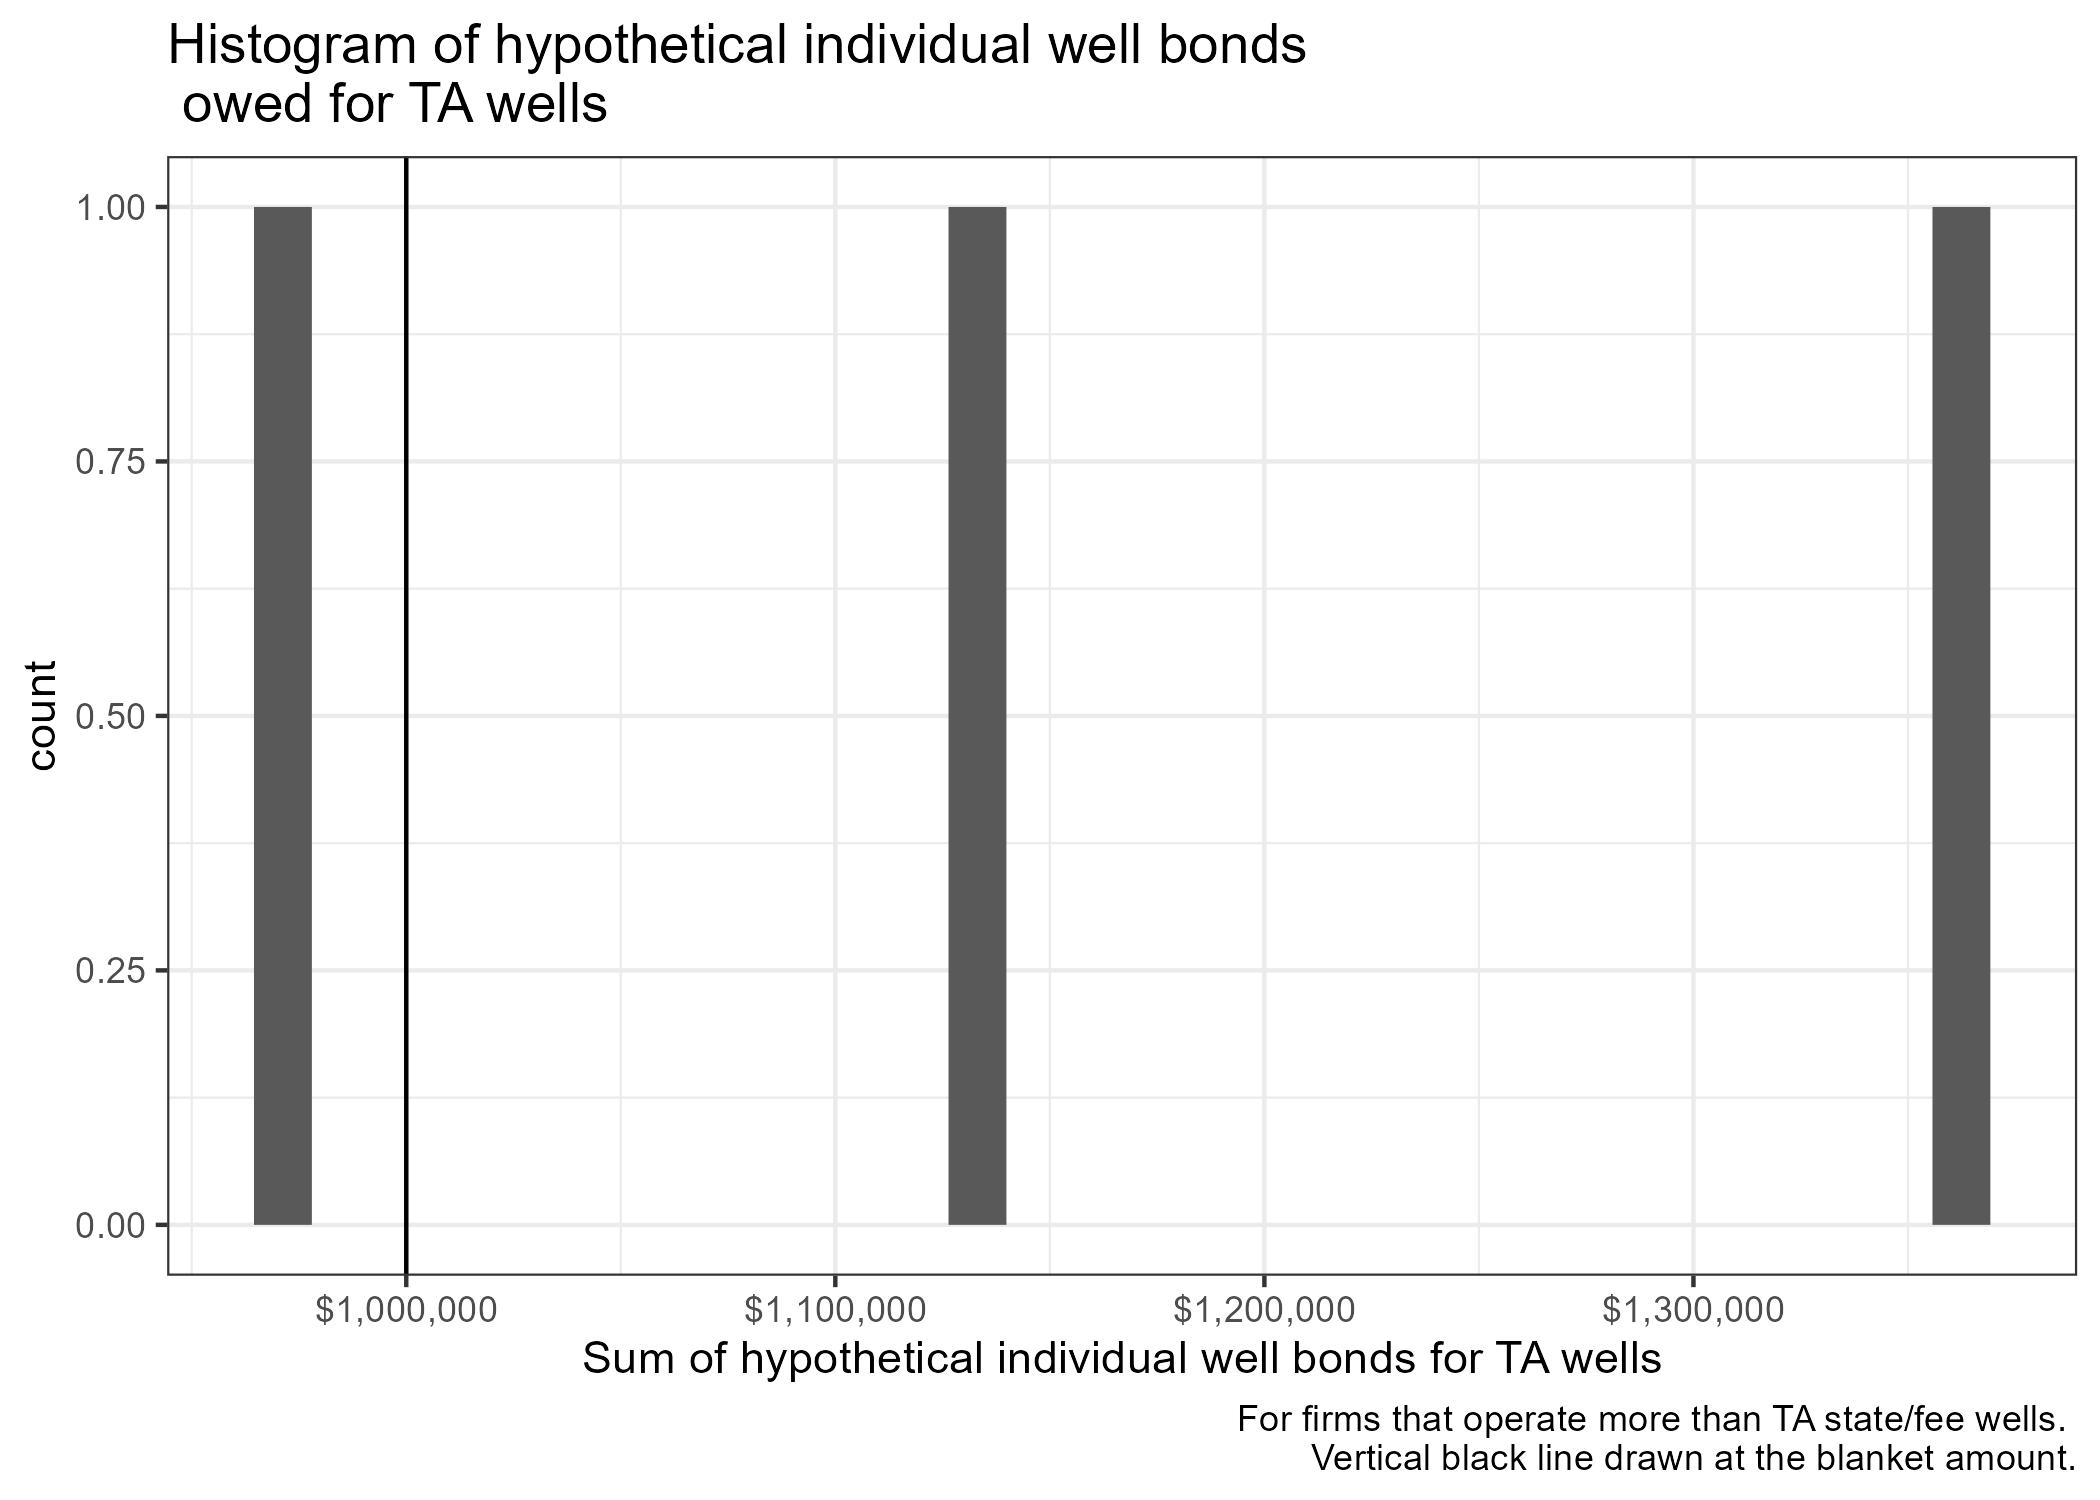
\includegraphics[width=0.45\linewidth]{Figures/Histogram_TA_25.jpg}
\end{tabular}
\end{frame}

\begin{frame}{Some blankets are more problematic than others}
\vspace{-1cm}
\begin{tabular}{cc}
    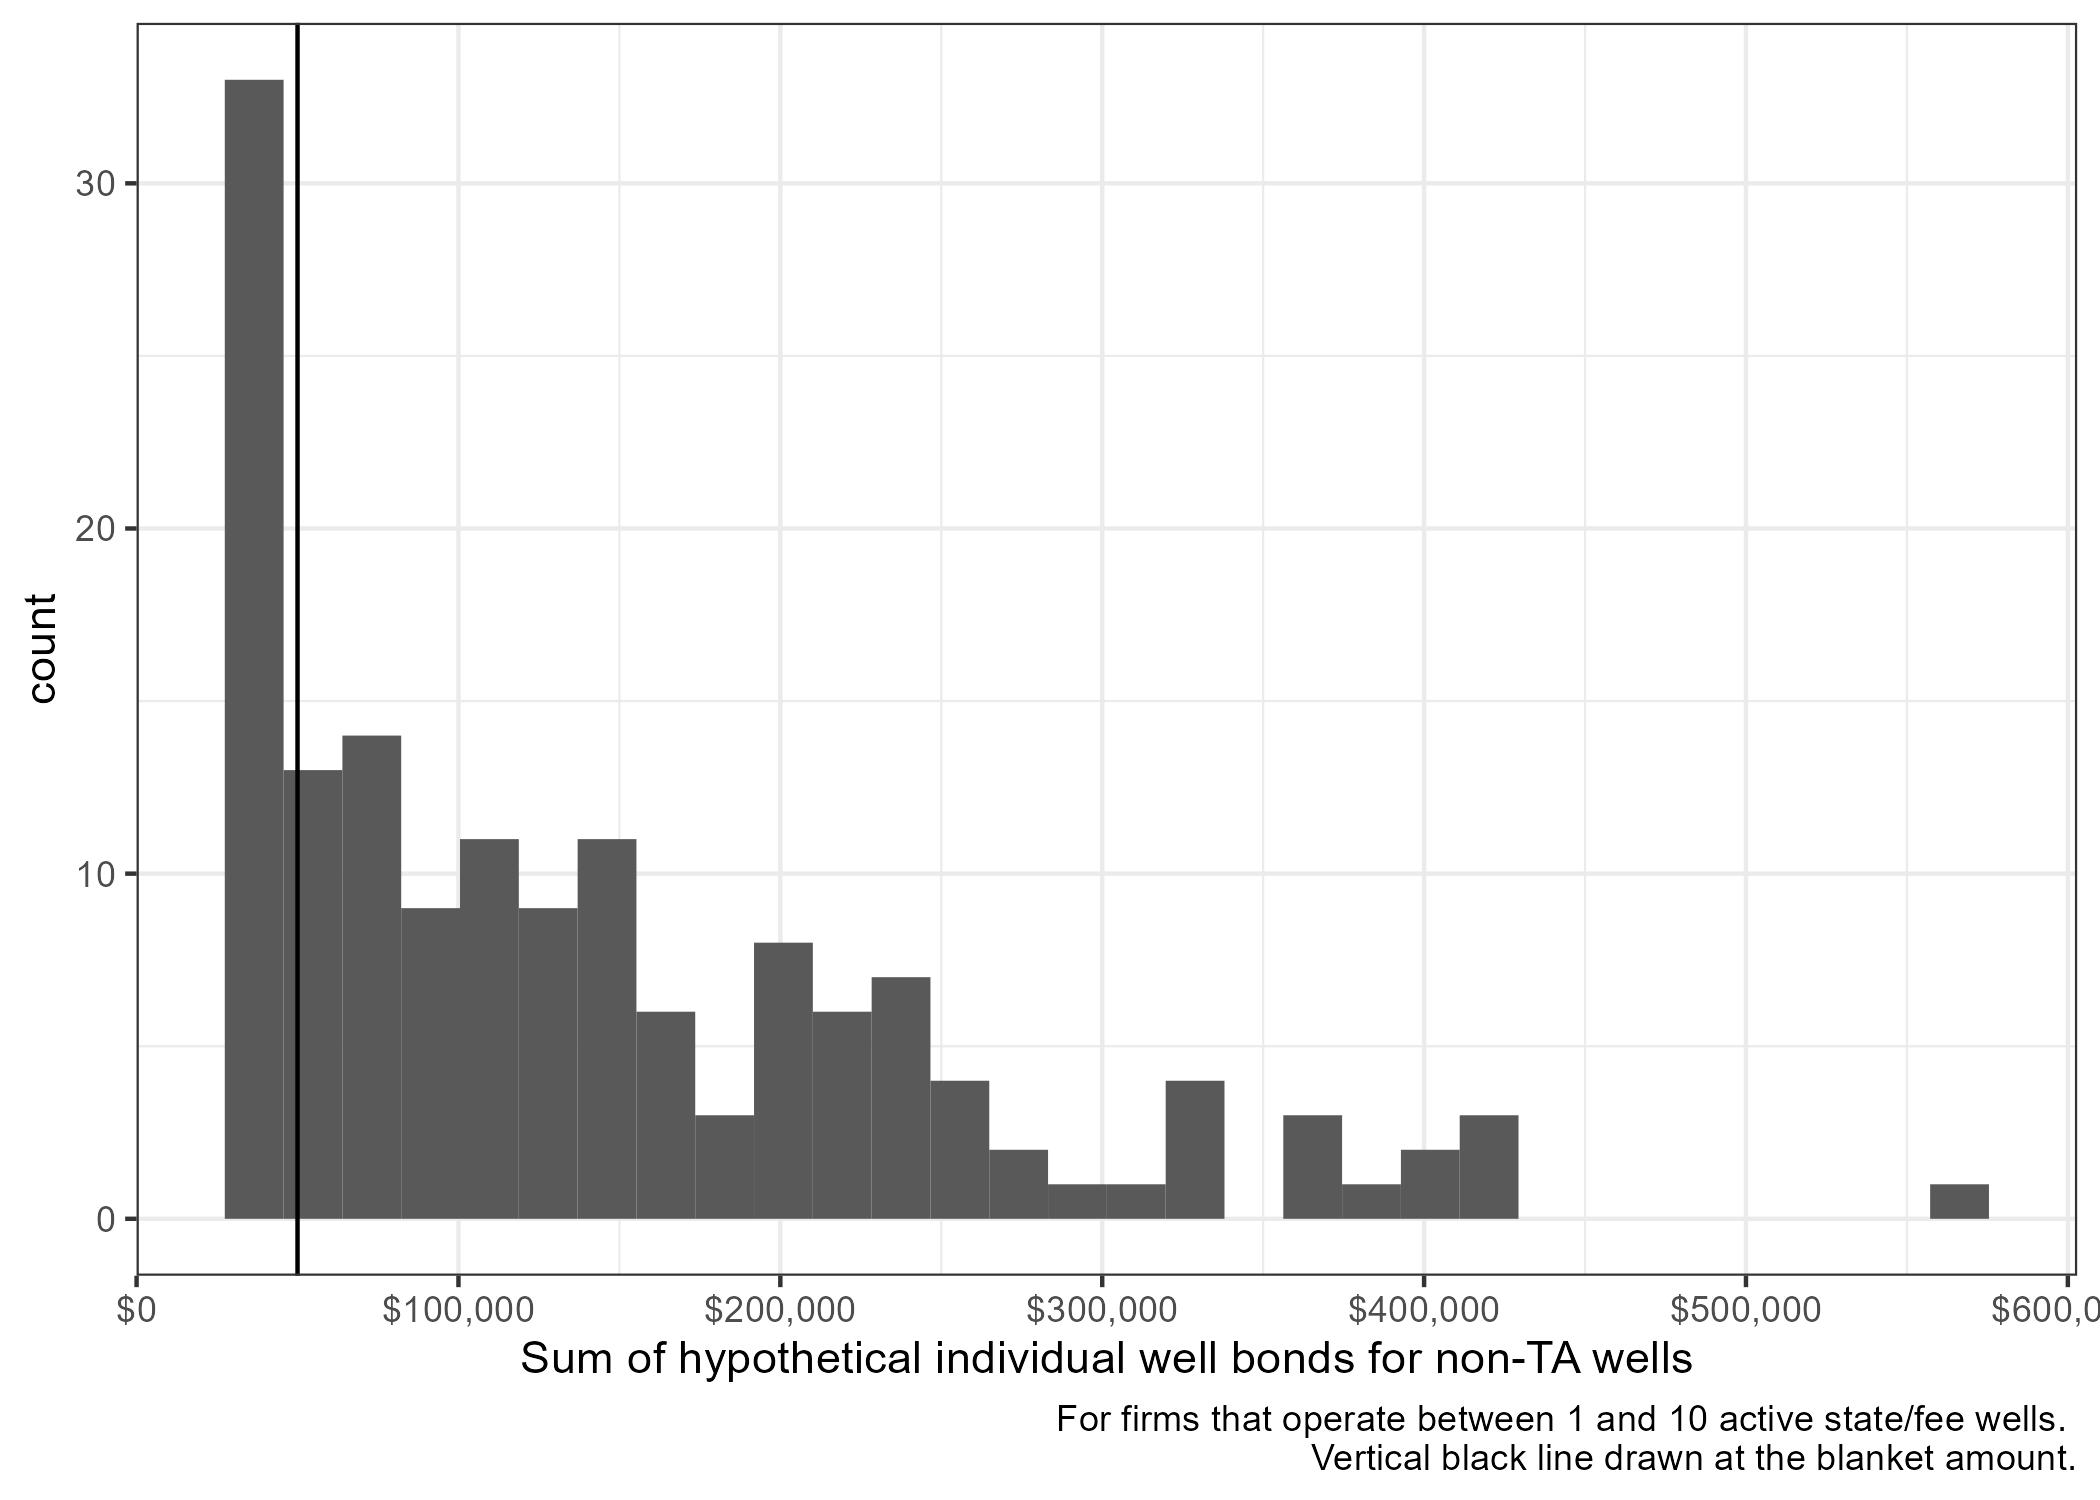
\includegraphics[width=0.45\linewidth]{Figures/Histogram_nonTA_1_10.jpg} & 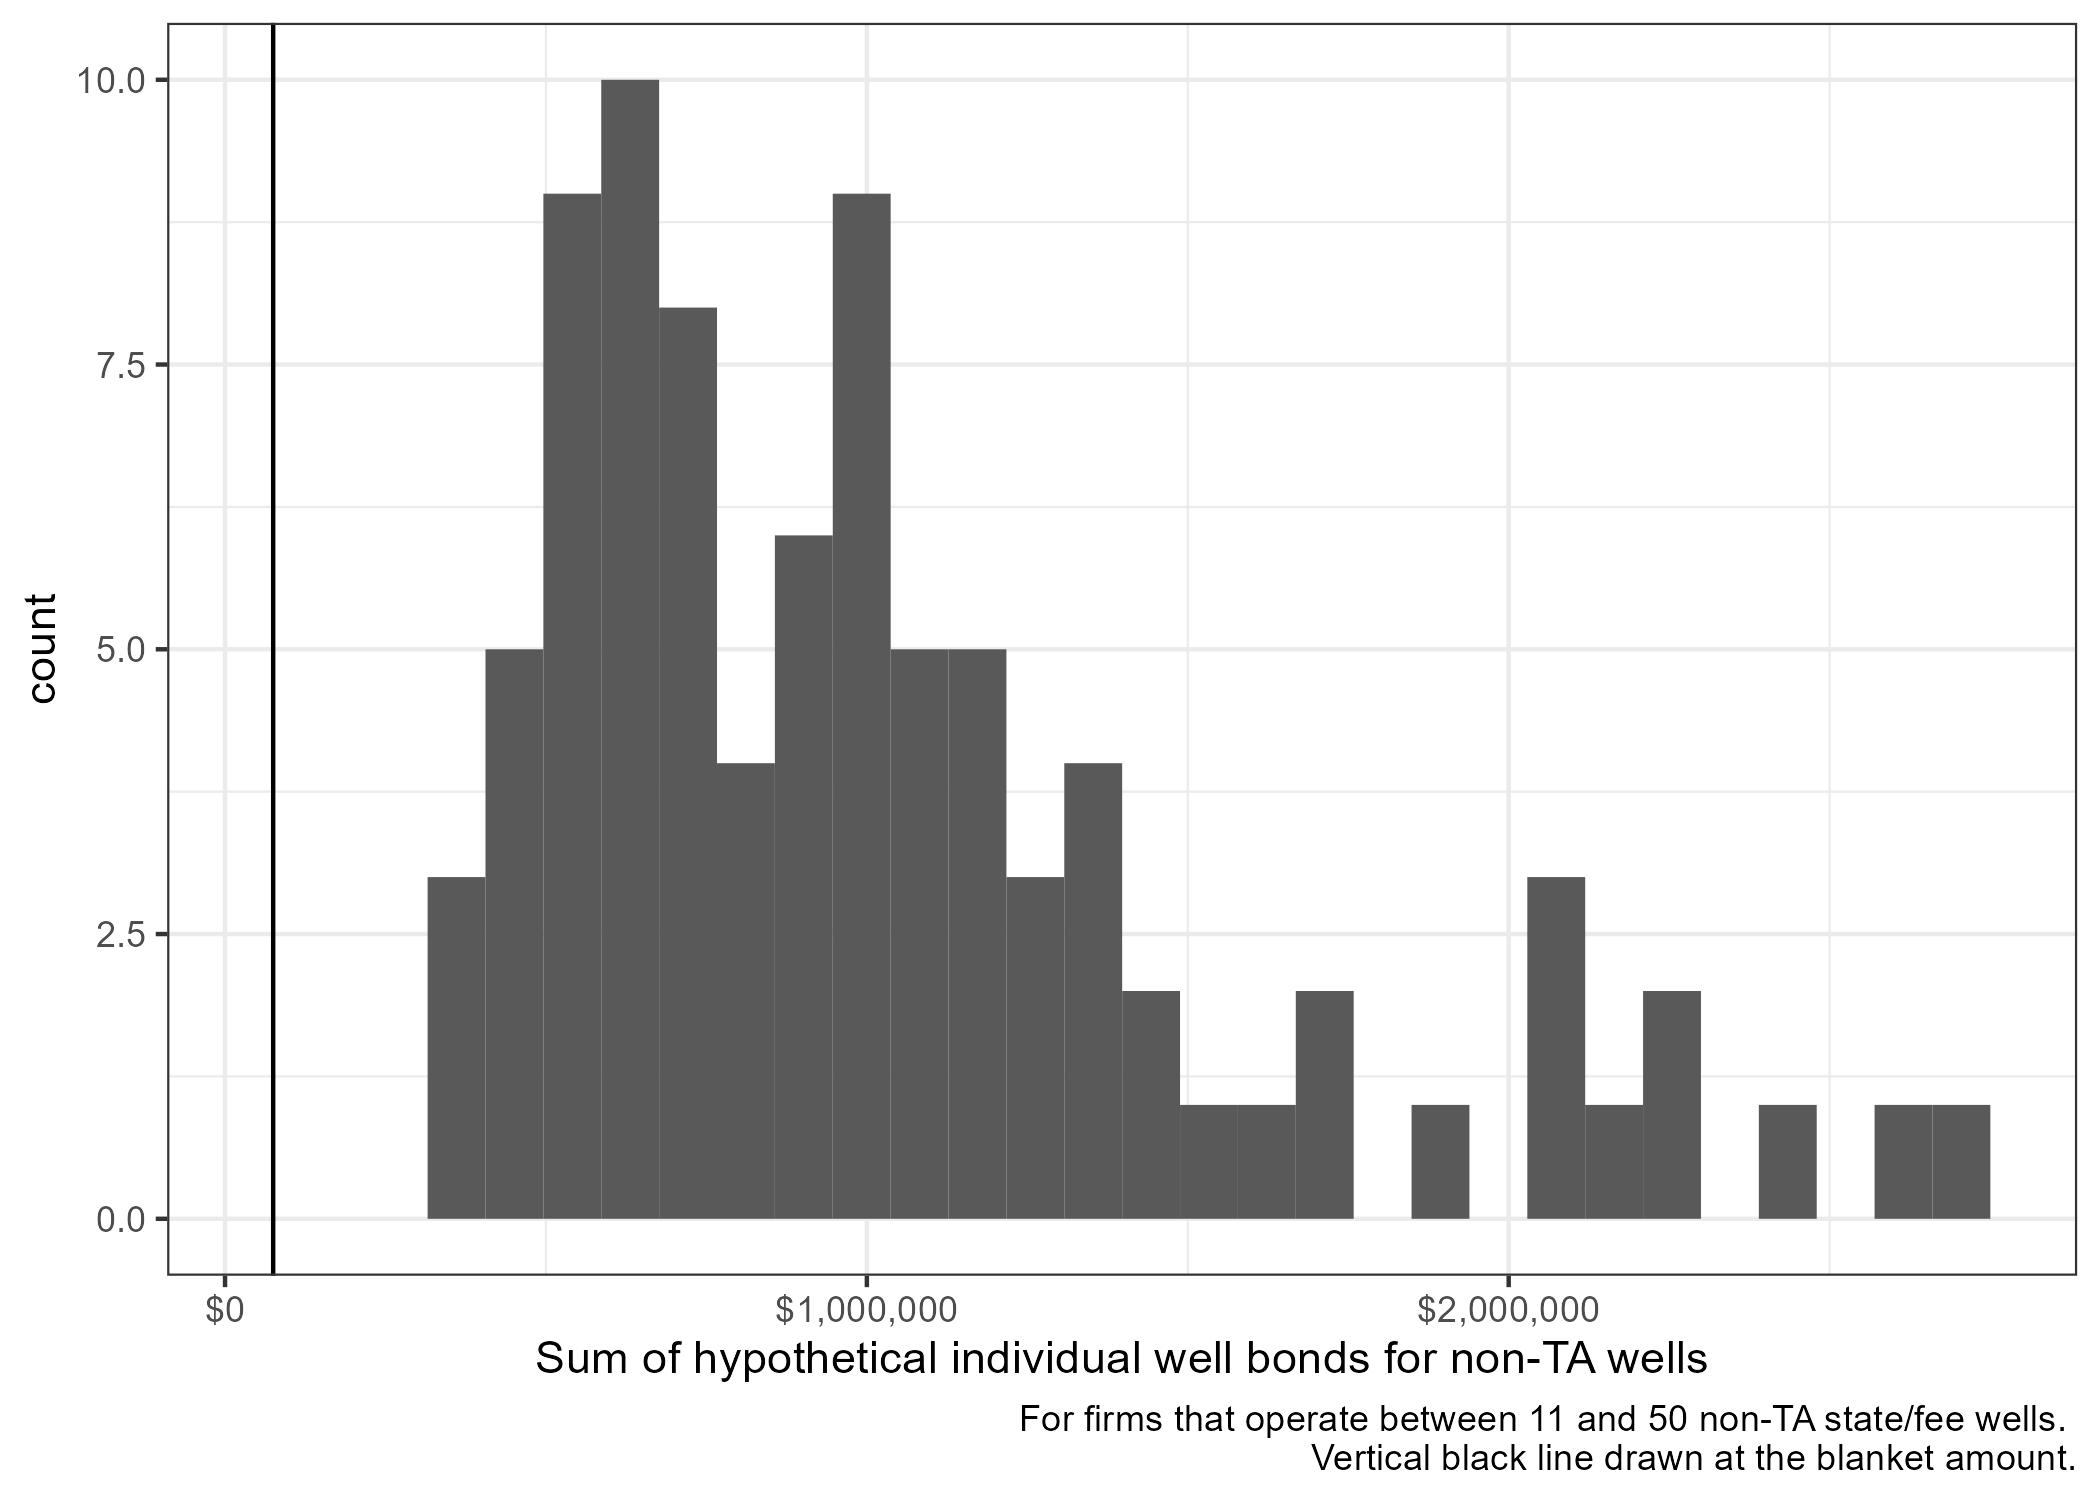
\includegraphics[width=0.45\linewidth]{Figures/Histogram_nonTA_11_50.jpg} \\
     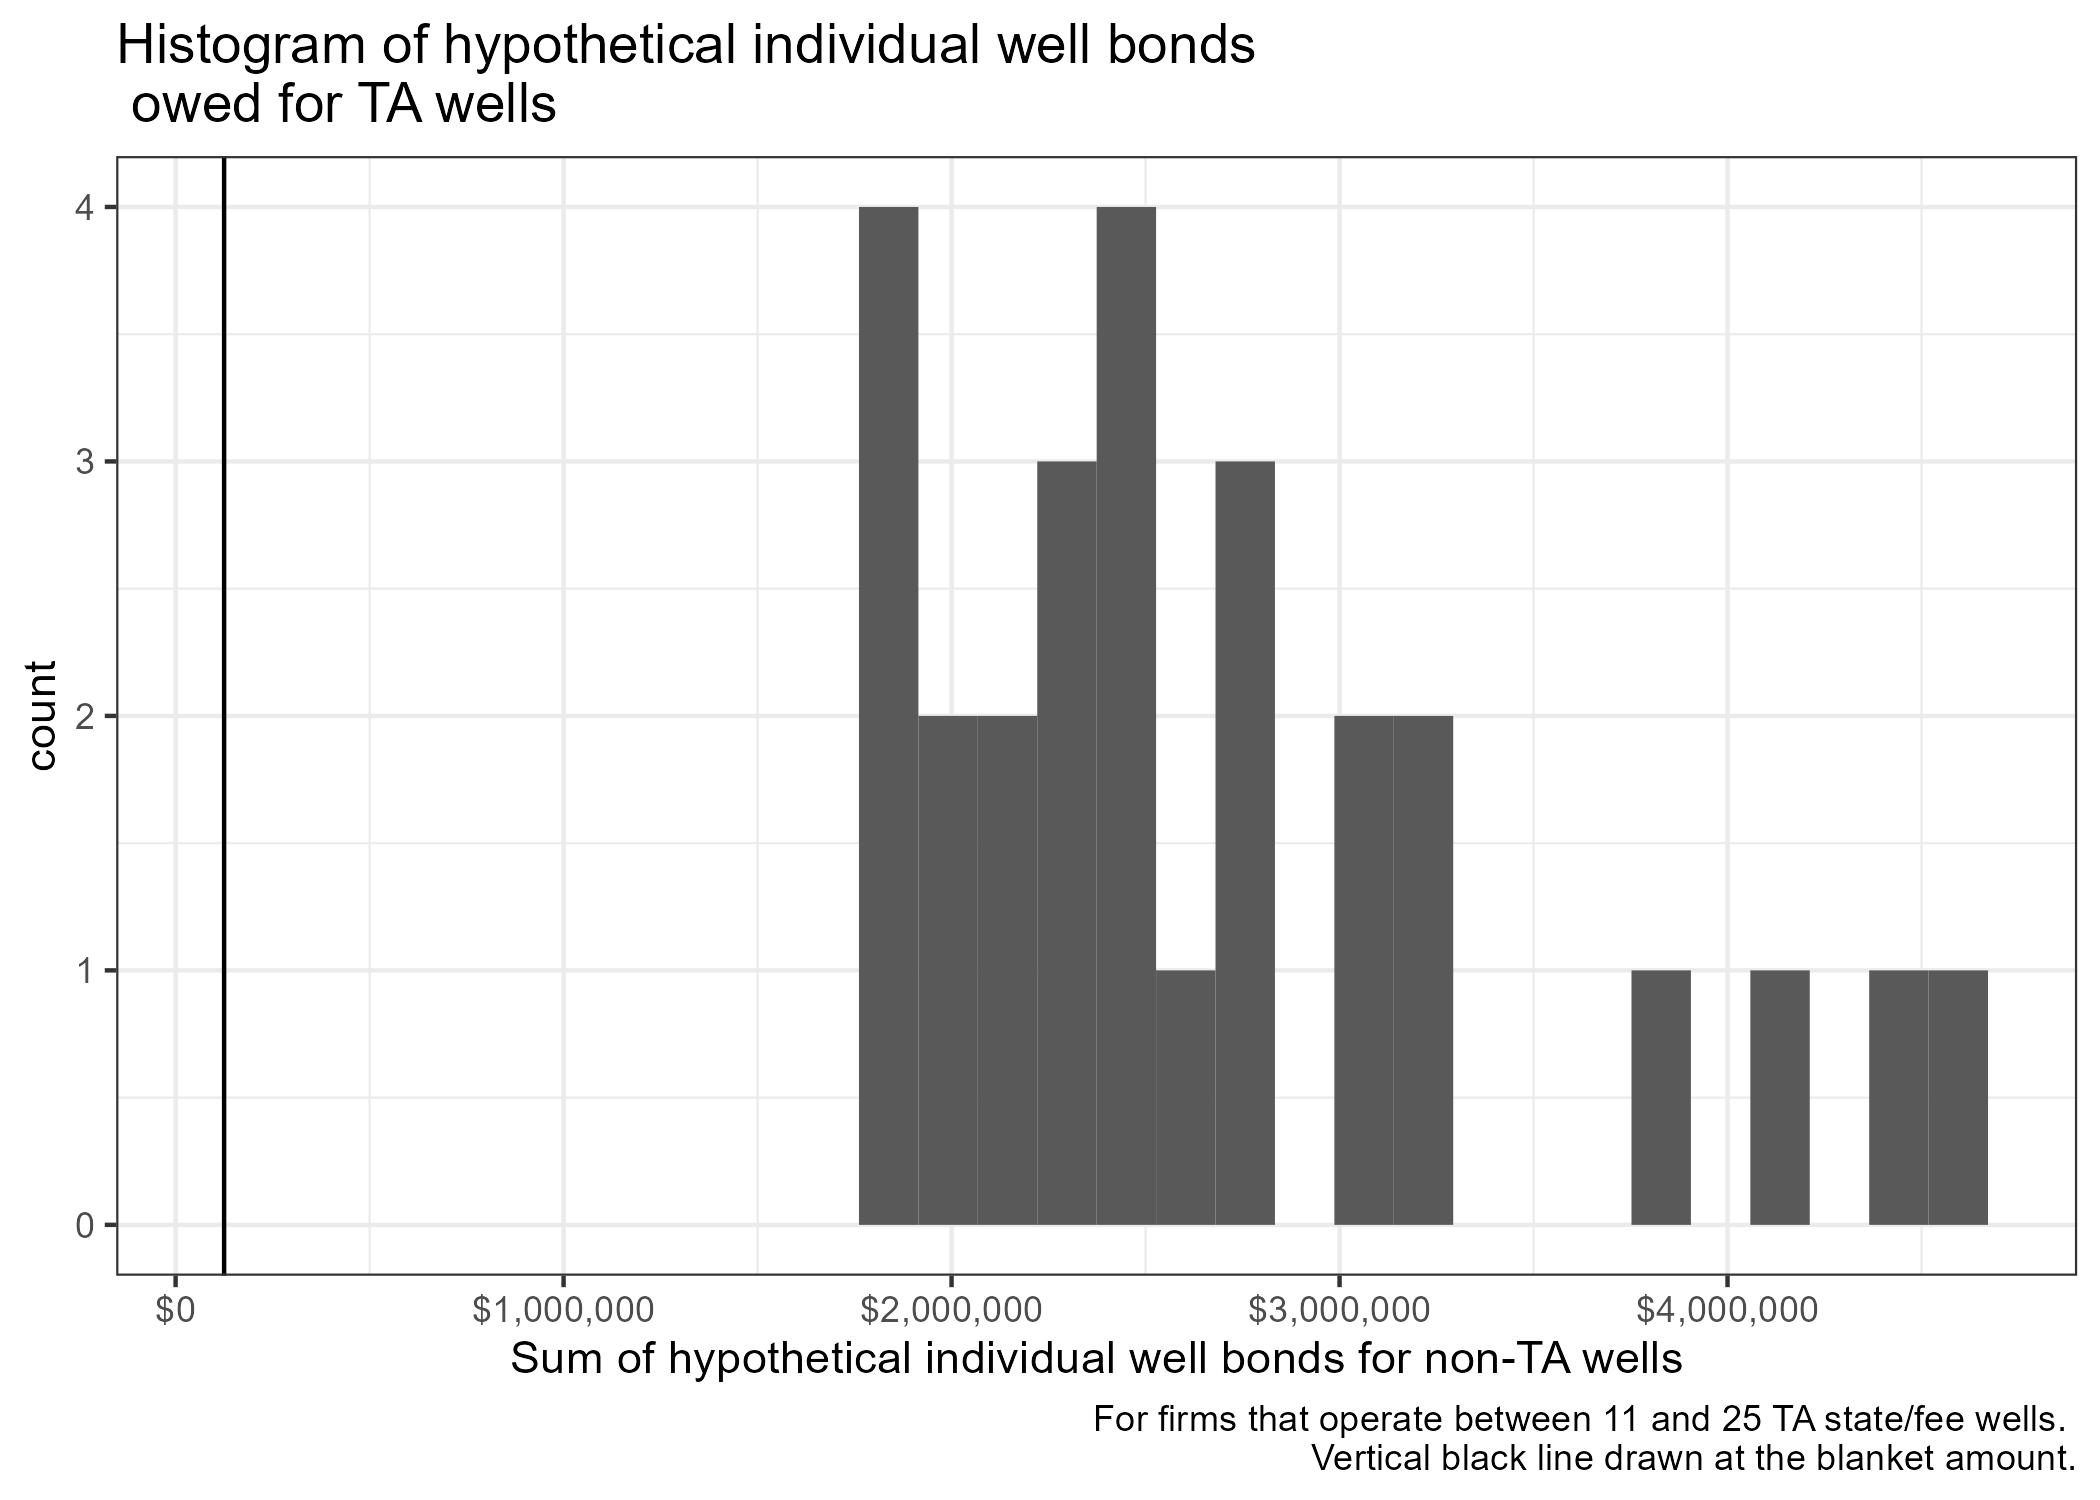
\includegraphics[width=0.45\linewidth]{Figures/Histogram_nonTA_51_100.jpg}& 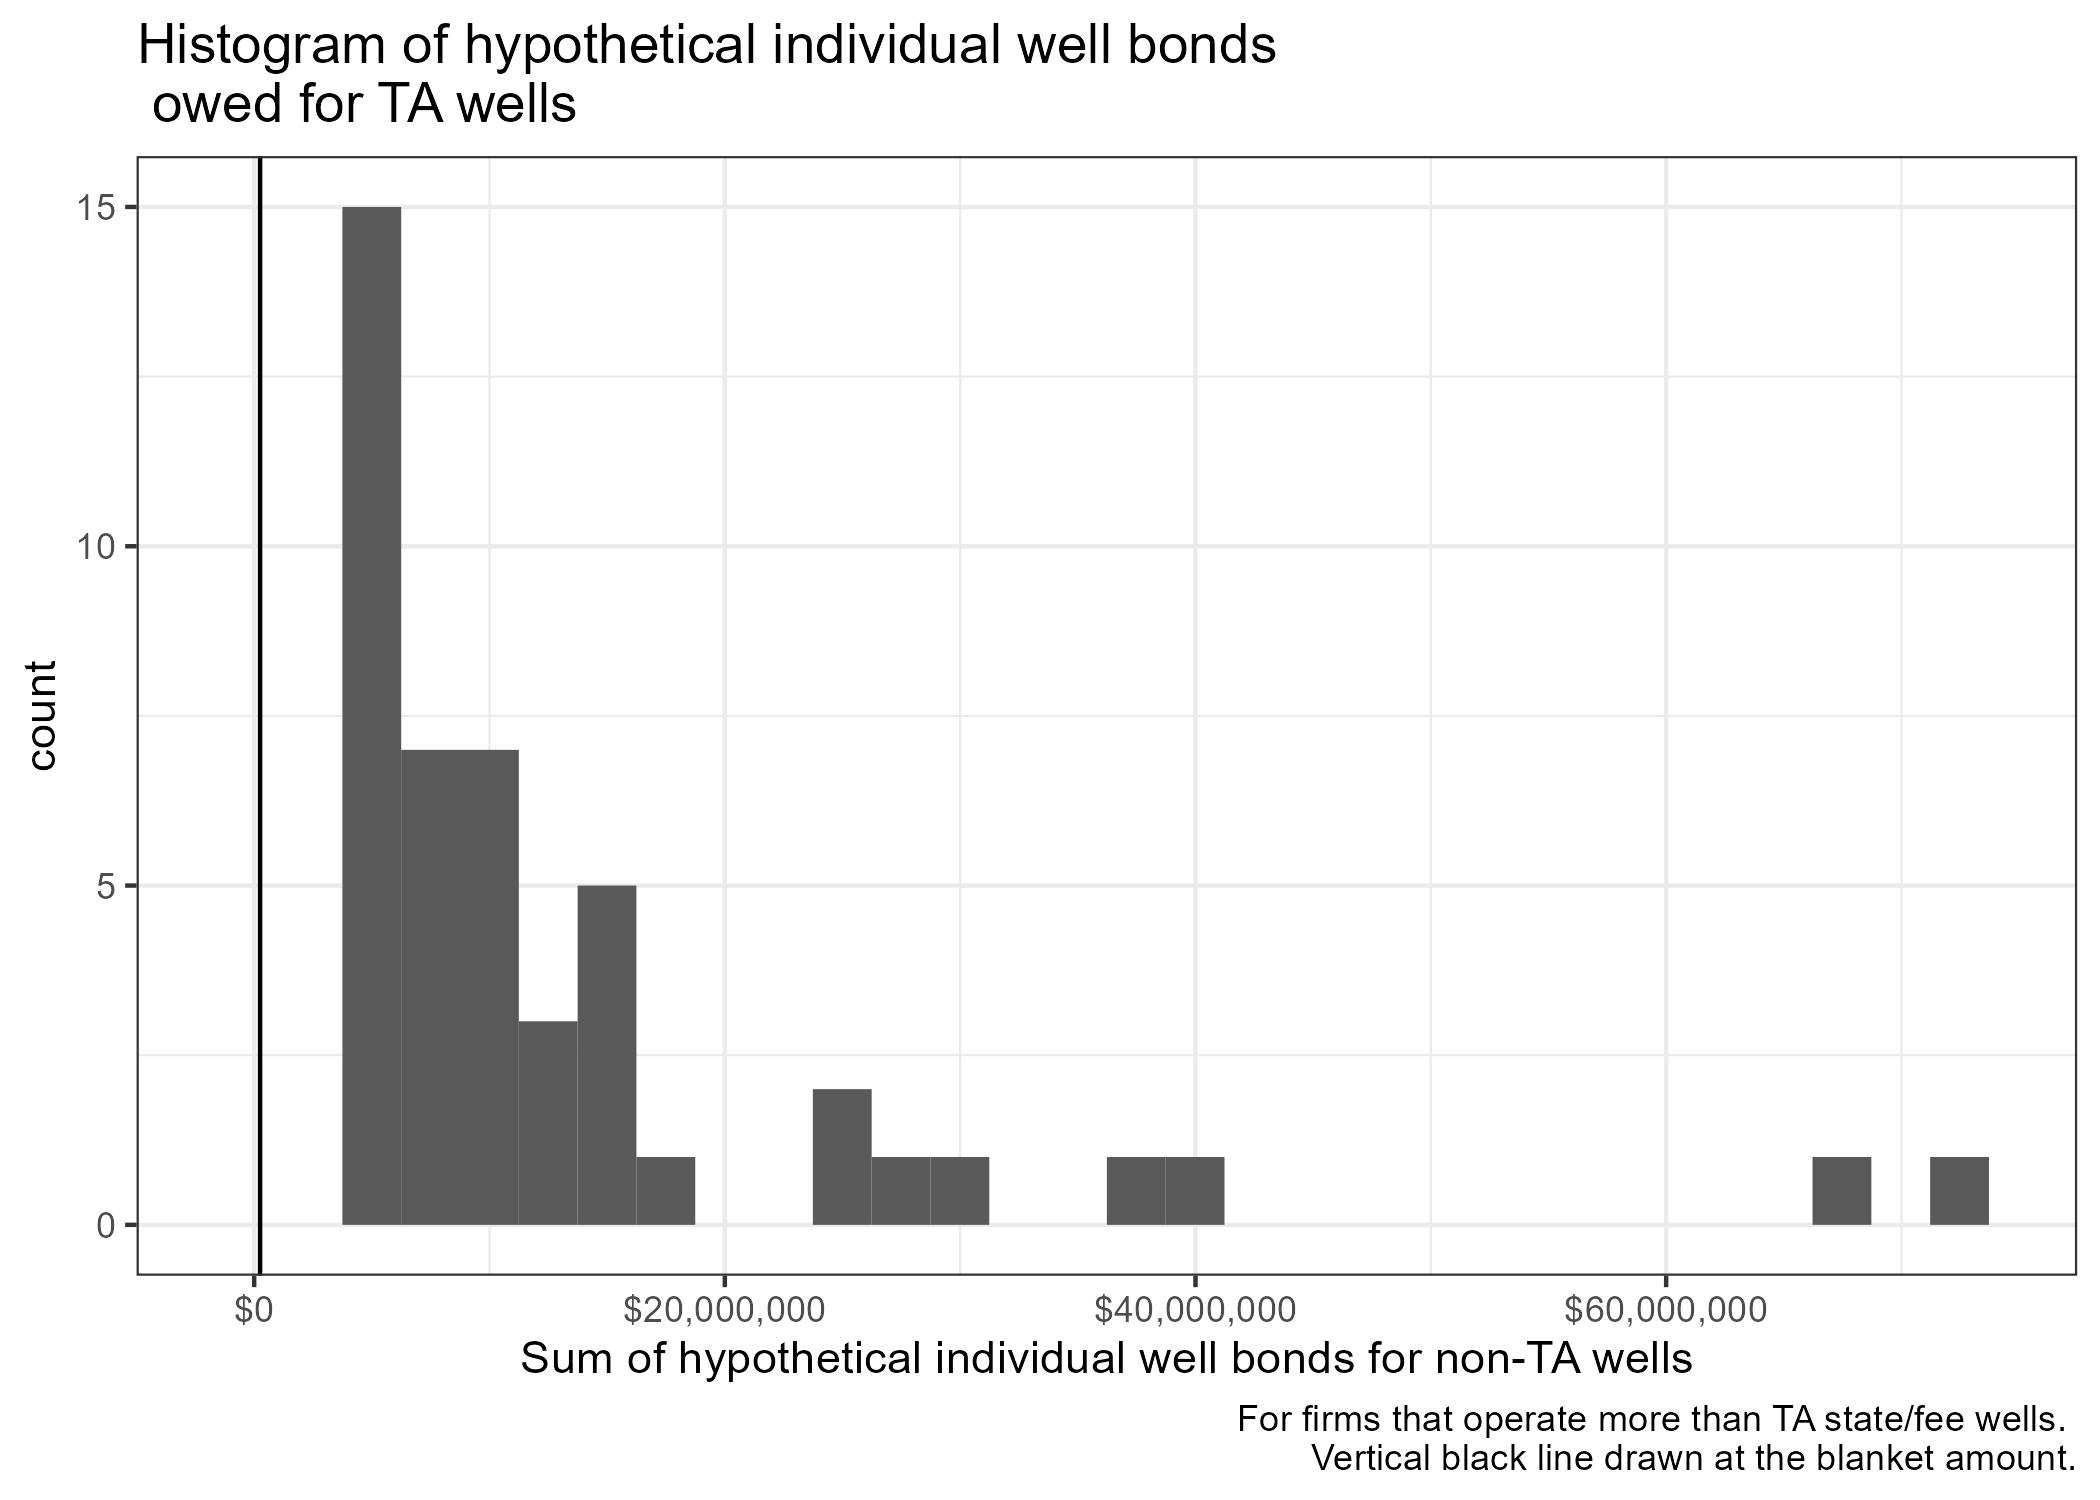
\includegraphics[width=0.45\linewidth]{Figures/Histogram_nonTA_100.jpg}
\end{tabular}
\end{frame}

\begin{frame}{Utah's New Bonding Proposal}
    \begin{itemize}
        \item Create tiers for operators based on total production and proportion of \textit{statewide} inactive wells.
        \item Firms that meet higher production requirements / lower inactive well proportions qualify for reduced bonding amounts.
        \item Bonds are also based upon average operator well depth.
        
    \end{itemize}
\end{frame}

\begin{frame}{Utah's Regulations Would Do a Great Job of Covering Plugging Liabilities in New Mexico}
\vspace{-0.5cm}
    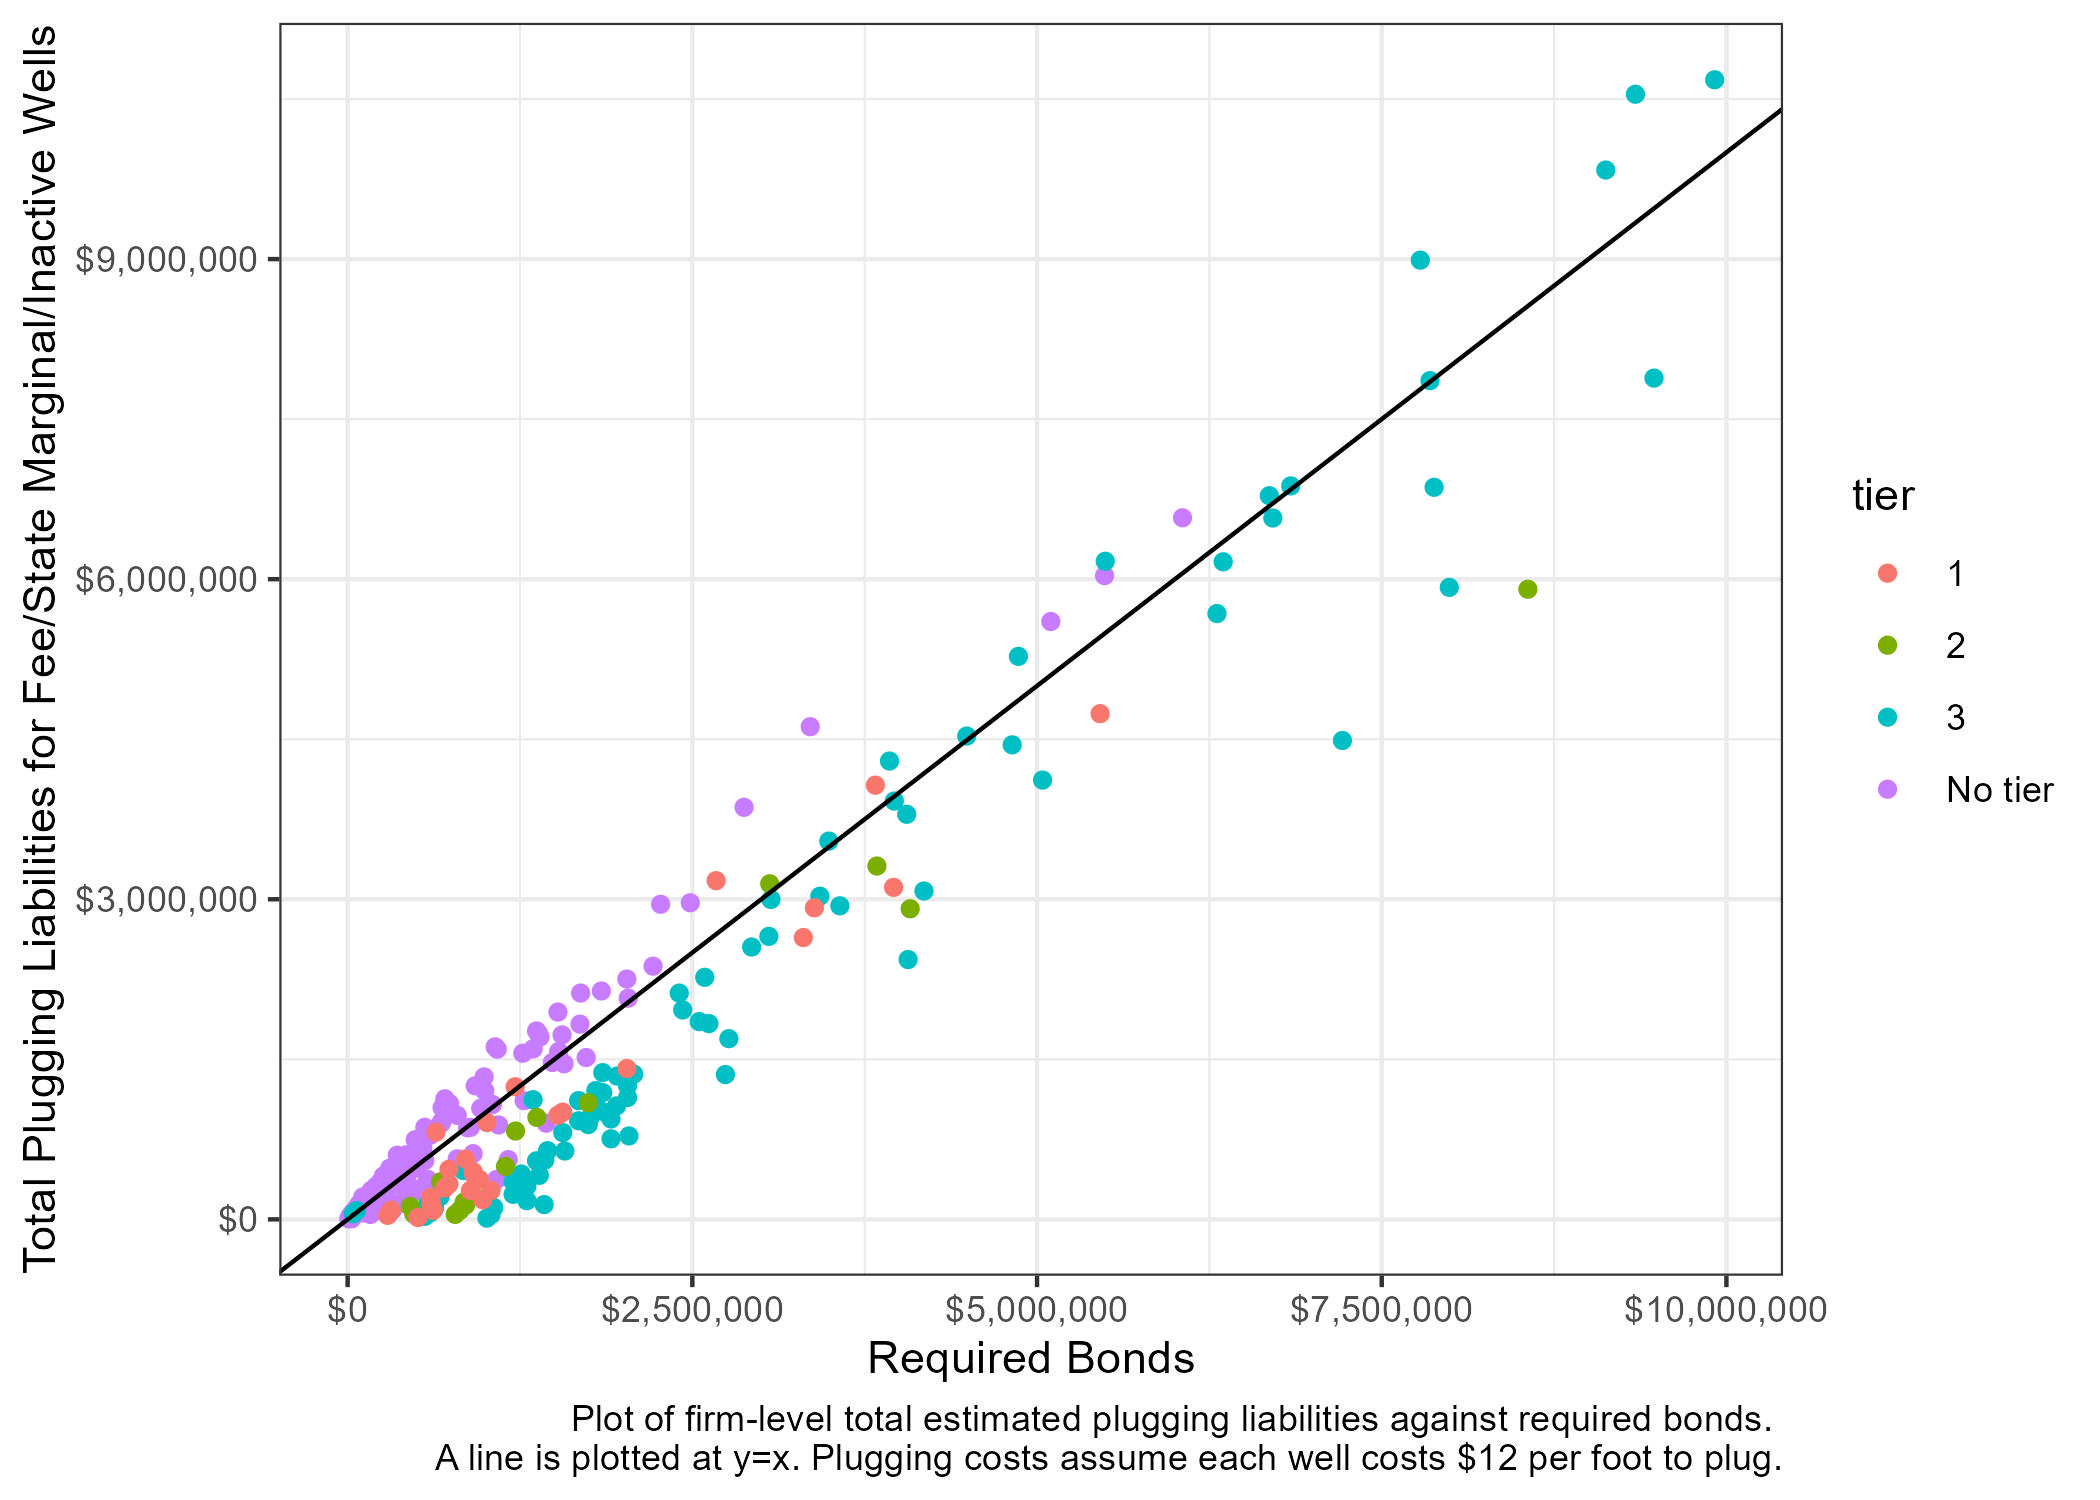
\includegraphics[width=0.8\textwidth]{Figures/UtahReg/BondLiability_MarginalInactiveFeeState.jpg}
\end{frame}

\begin{frame}{Thanks!}
\label{Thanks}
    All of the code to reproduce these charts is available at: \href{https://github.com/lbeatty1/NewMexicoAnalytics}{https://github.com/lbeatty1/NewMexicoAnalytics}\\
    \vspace{1cm}


    Please feel free to contact me at:
    \href{mailto:lbeatty@edf.org}{lbeatty@edf.org}\\
    \vspace{1cm}

\end{frame}




\end{document}